\documentclass[12pt,letterpaper]{report}

% Packages
\usepackage[margin=1in]{geometry}
\usepackage{graphicx}
\usepackage{booktabs}
\usepackage{amsmath}
\usepackage{amssymb}
\usepackage[round]{natbib}
\usepackage{setspace}
\usepackage{listings}
\usepackage{xcolor}
\usepackage{caption}
\usepackage{subcaption}
\usepackage{float}
\usepackage{tabularx}
\usepackage{multirow}
\usepackage{enumitem}
\usepackage{appendix}
\usepackage{microtype}
\usepackage[hyphens]{url}
\usepackage[hidelinks]{hyperref}

% Double spacing for thesis
\doublespacing

% Fix page numbering for front matter
\pagenumbering{roman}

% Allow slightly loose spacing to prevent overfull boxes
\sloppy

% Code listing style
\lstset{
  basicstyle=\ttfamily\small,
  breaklines=true,
  frame=single,
  backgroundcolor=\color{gray!5},
  keywordstyle=\color{blue},
  commentstyle=\color{green!50!black},
}

% Figure path
\graphicspath{{figures/}}

% ============================================================
% TITLE PAGE
% ============================================================
\begin{document}

\begin{titlepage}
\centering
\vspace*{2cm}

{\LARGE \textbf{Navigation-Driven Evaluation of 2D LiDAR SLAM:\\
A Comparative Study of SLAM Toolbox and Cartographer\\
in Autonomous Rover Missions}}

\vspace{2cm}

{\large A Thesis Submitted in Partial Fulfillment\\
of the Requirements for the Degree of\\
\textbf{Master of Science}}

\vspace{2cm}

{\large by\\
\textbf{Zamin Anwar}}

\vspace{3cm}

{\large \the\year}

\vfill
\end{titlepage}

% ============================================================
% ABSTRACT
% ============================================================
\begin{abstract}
\addcontentsline{toc}{chapter}{Abstract}

Simultaneous Localization and Mapping (SLAM) is a foundational capability for autonomous mobile robots, yet selecting between available algorithms remains challenging for practitioners. Traditional SLAM benchmarks evaluate trajectory accuracy in isolation, without examining how accuracy differences affect downstream task performance. This thesis presents a navigation-driven evaluation framework that compares two widely deployed 2D LiDAR SLAM algorithms---SLAM Toolbox and Google Cartographer---through the lens of autonomous navigation using the Nav2 framework on a simulated differential-drive rover.

We developed a reproducible experimental platform using Gazebo Harmonic and ROS~2 Jazzy that integrates SLAM-in-the-loop with Nav2 for closed-loop autonomous navigation. Ground truth is obtained directly from the simulator through a dedicated transform tree that avoids interference with the SLAM coordinate frames. Three navigation goal sets of increasing complexity were designed to test algorithm performance across varying trajectory lengths (12--35\,m) and turning demands.

Experiments comprising 18~runs (2~algorithms $\times$ 3~goal sets $\times$ 3~repetitions) reveal that both algorithms achieve 100\% navigation success across all conditions. However, SLAM Toolbox demonstrates 6--11$\times$ lower Absolute Trajectory Error (ATE), with mean RMSE values of 0.96--2.84\,cm compared to Cartographer's 10.82--18.09\,cm. Relative Pose Error differences are smaller (1.7--3$\times$), indicating the accuracy gap is primarily in global consistency rather than local scan matching. Notably, the substantial accuracy difference produces no measurable difference in navigation success or mission completion time.

These findings suggest that current SLAM accuracy benchmarks may overemphasize trajectory precision beyond task-relevant thresholds, and that navigation-driven evaluation offers a complementary perspective for algorithm selection. The complete experimental framework is released as open-source software.

\end{abstract}

% ============================================================
% FRONT MATTER
% ============================================================
\tableofcontents
\listoffigures
\listoftables

% ============================================================
% CHAPTERS
% ============================================================
\pagenumbering{arabic}
\chapter{Introduction}
\label{ch:introduction}

\section{Motivation}

Autonomous mobile robots are increasingly deployed in warehouses, hospitals, agricultural fields, and urban environments. A fundamental requirement for any mobile robot operating without external positioning infrastructure is the ability to simultaneously determine its own location and construct a representation of its surroundings---a problem known as Simultaneous Localization and Mapping (SLAM) \citep{thrun2005probabilistic}. Over the past two decades, the SLAM problem has received extensive attention from the robotics research community, resulting in a rich ecosystem of algorithms spanning different sensor modalities, mathematical formulations, and computational trade-offs \citep{grisetti2010gmapping, dellaert2017factor}.

For 2D LiDAR-equipped ground robots---a common configuration in indoor service robotics, warehouse automation, and research platforms---two algorithms have emerged as particularly prominent open-source solutions within the Robot Operating System (ROS) ecosystem: SLAM Toolbox \citep{macenski2021slam} and Google Cartographer \citep{hess2016cartographer}. Both are actively maintained, widely deployed, and represent different architectural approaches to the same problem. SLAM Toolbox employs a continuous pose graph with Ceres-based optimization, while Cartographer uses a submap-based approach with branch-and-bound loop closure detection. Despite their popularity, practitioners frequently face difficulty choosing between them, as the relative merits depend heavily on the deployment context.

Traditional SLAM evaluation methodologies, established by influential benchmarks such as the TUM RGB-D dataset \citep{sturm2012benchmark} and the KITTI odometry benchmark \citep{geiger2013kitti}, focus on trajectory accuracy metrics---primarily Absolute Trajectory Error (ATE) and Relative Pose Error (RPE). These metrics provide a rigorous quantitative assessment of localization quality but are computed in an open-loop fashion: the SLAM algorithm processes pre-recorded sensor data, and its estimated trajectory is compared against ground truth. This evaluation paradigm, while valuable, does not capture how localization errors propagate through a complete autonomous system. In practice, SLAM provides localization for a navigation stack that plans paths, avoids obstacles, and controls the robot in a closed feedback loop. The question of whether a measurable difference in SLAM trajectory accuracy translates to a meaningful difference in navigation performance remains largely unexamined.

The emergence of Nav2 \citep{macenski2020nav2} as the standard navigation framework for ROS~2 provides an opportunity to bridge this gap. Nav2 offers a modular, production-quality navigation stack that integrates global and local planning, obstacle avoidance, and recovery behaviors. By operating Nav2 with SLAM-in-the-loop---where the SLAM algorithm provides real-time localization to the navigation stack---we can evaluate SLAM algorithms not only on their trajectory accuracy but also on their impact on task-level performance.

\section{Problem Statement}

This thesis addresses the following overarching question: \emph{How do 2D LiDAR SLAM algorithms compare when evaluated through the lens of autonomous navigation task performance, rather than trajectory accuracy alone?}

Specifically, we investigate whether the accuracy differences observed between SLAM Toolbox and Cartographer in traditional benchmarks translate to meaningful differences in closed-loop navigation outcomes. We conduct this investigation in a simulation environment using Gazebo Harmonic with ROS~2 Jazzy, where ground truth is available from the simulator and experimental conditions can be precisely controlled and repeated.

\section{Research Questions}

This thesis seeks to answer the following research questions:

\begin{description}[style=nextline]
\item[RQ1:] How do SLAM Toolbox and Cartographer compare in SLAM accuracy (ATE and RPE) across navigation trajectories of varying complexity?
\item[RQ2:] Does SLAM accuracy predict autonomous navigation success rate and mission efficiency in closed-loop Nav2 missions?
\item[RQ3:] How do the two algorithms scale in accuracy and performance as trajectory length and navigational complexity increase?
\end{description}

\section{Contributions}

This thesis makes the following contributions:

\begin{enumerate}
\item \textbf{A reproducible SLAM-in-the-loop navigation evaluation framework.} We develop an open-source experimental platform that integrates Gazebo Harmonic simulation, ROS~2 Jazzy, and the Nav2 navigation stack to evaluate SLAM algorithms through autonomous navigation task performance. The framework includes automated experiment orchestration, ground truth collection through a dedicated transform tree, and standardized metric computation.

\item \textbf{A quantitative comparison across three complexity levels with statistical validation.} We present experimental results from 18 trials (2 algorithms $\times$ 3 goal sets $\times$ 3 repetitions) comparing SLAM Toolbox and Cartographer on trajectory accuracy (ATE, RPE), navigation success rate, and mission completion time. Results are reported with mean and standard deviation to support statistical interpretation.

\item \textbf{An analysis of the accuracy--utility gap in SLAM-based navigation.} We provide empirical evidence that a 6--11$\times$ difference in SLAM trajectory accuracy produces no measurable difference in navigation success rate or mission time within our experimental conditions, suggesting that traditional accuracy benchmarks may overemphasize precision beyond task-relevant thresholds.

\item \textbf{Open-source software.} The complete experimental framework, including robot model, simulation environment, SLAM configurations, navigation integration, experiment orchestration scripts, and analysis tools, is released as open-source software to facilitate reproduction and extension.
\end{enumerate}

\section{Thesis Structure}

The remainder of this thesis is organized as follows:

\begin{description}[style=nextline]
\item[Chapter~\ref{ch:background}] provides background on SLAM fundamentals, the two algorithms under study, the Nav2 navigation framework, and established evaluation methodology. It also reviews related benchmarking work and identifies the research gap addressed by this thesis.
\item[Chapter~\ref{ch:methodology}] describes the experimental methodology, including the simulation platform, robot model, SLAM and navigation configurations, experimental design with three goal sets of increasing complexity, and the evaluation metrics employed.
\item[Chapter~\ref{ch:implementation}] details the software implementation, covering the ROS~2 package architecture, transform frame design, experiment orchestration pipeline, and key technical challenges encountered and resolved.
\item[Chapter~\ref{ch:results}] presents the experimental results across all 18 trials, including navigation success rates, SLAM accuracy metrics, mission timing, scaling behavior, and run-to-run consistency.
\item[Chapter~\ref{ch:discussion}] interprets the results in the context of the research questions, analyzes the accuracy--utility gap, discusses algorithmic explanations for the observed differences, and acknowledges limitations.
\item[Chapter~\ref{ch:conclusion}] summarizes the contributions and findings, and outlines directions for future work.
\end{description}

\chapter{Background and Related Work}
\label{ch:background}

\section{Simultaneous Localization and Mapping}

The SLAM problem requires a robot to incrementally build a map of an unknown environment while simultaneously using that map to determine its own position \citep{thrun2005probabilistic}. This circular dependency---accurate mapping requires accurate localization, and accurate localization requires an accurate map---makes SLAM one of the fundamental challenges in mobile robotics.

\subsection{Problem Formulation}

Formally, the SLAM problem can be stated as follows. Given a sequence of sensor observations $z_{1:t} = \{z_1, z_2, \ldots, z_t\}$ and control inputs $u_{1:t} = \{u_1, u_2, \ldots, u_t\}$, estimate the posterior probability of the robot's trajectory $x_{0:t} = \{x_0, x_1, \ldots, x_t\}$ and the map $m$:
\begin{equation}
p(x_{0:t}, m \mid z_{1:t}, u_{1:t})
\end{equation}
This joint estimation problem can be decomposed and solved through various mathematical frameworks, broadly categorized as filter-based and graph-based approaches.

\subsection{Filter-Based Approaches}

Early SLAM solutions employed recursive Bayesian filtering. The Extended Kalman Filter (EKF) SLAM algorithm maintains a joint Gaussian distribution over the robot state and landmark positions, updating both with each new observation. While mathematically elegant, EKF-SLAM suffers from quadratic computational complexity in the number of landmarks, limiting its scalability.

Particle filter approaches, such as Rao-Blackwellized particle filters used in GMapping \citep{grisetti2010gmapping}, represent the posterior distribution using a set of weighted particles. Each particle carries a robot trajectory hypothesis and an associated map. Adaptive techniques such as KLD-sampling \citep{fox2003kld} reduce computational cost by adjusting the number of particles based on the complexity of the posterior distribution.

\subsection{Graph-Based Approaches}

Modern SLAM systems predominantly employ graph-based formulations \citep{grisetti2010gmapping, dellaert2017factor}. In this framework, robot poses are represented as nodes in a graph, and spatial constraints between poses---derived from odometry, scan matching, or loop closure detection---are represented as edges. The SLAM problem reduces to a nonlinear least-squares optimization:
\begin{equation}
x^* = \arg\min_x \sum_{(i,j) \in \mathcal{E}} \| e_{ij}(x_i, x_j) \|^2_{\Omega_{ij}}
\end{equation}
where $e_{ij}$ is the error function for the constraint between poses $x_i$ and $x_j$, and $\Omega_{ij}$ is the information matrix encoding constraint uncertainty. Efficient solvers such as g2o \citep{kummerle2011g2o} and Ceres Solver \citep{agarwal2010ceres} make this optimization tractable for large pose graphs.

\subsection{The 2D LiDAR SLAM Landscape}

Two-dimensional LiDAR sensors provide planar range measurements that are well-suited for indoor and structured environments. The 2D SLAM landscape includes several prominent algorithms: GMapping (particle filter-based), Hector SLAM \citep{kohlbrecher2011hector} (scan matching without odometry), Cartographer \citep{hess2016cartographer} (submap-based with branch-and-bound loop closure), and SLAM Toolbox \citep{macenski2021slam} (pose graph with Ceres optimization). This thesis focuses on the latter two as the most actively maintained and widely deployed solutions in the ROS~2 ecosystem.

\section{SLAM Toolbox}

SLAM Toolbox \citep{macenski2021slam} is an open-source SLAM library designed for production deployment in dynamic, real-world environments. Developed as a successor to the earlier Karto SLAM library, it provides a graph-based SLAM solution with several operational modes.

\subsection{Architecture}

SLAM Toolbox maintains a pose graph where each node represents a robot pose associated with a laser scan. Edges encode spatial constraints derived from scan matching between consecutive poses (sequential constraints) and between non-adjacent poses that observe the same region (loop closure constraints). The pose graph is optimized using the Ceres Solver \citep{agarwal2010ceres}, a widely used nonlinear least-squares optimization library developed by Google.

The system operates in multiple modes: \emph{synchronous} mode processes each incoming scan sequentially, \emph{asynchronous} mode allows scans to be processed at a rate independent of acquisition, and \emph{localization} mode operates on a pre-built map. For real-time SLAM applications, asynchronous mode is typically preferred as it decouples scan processing from the sensor data rate.

\subsection{Scan Matching and Loop Closure}

Local scan matching in SLAM Toolbox uses a correlative scan matcher followed by Ceres-based refinement. When a new scan is acquired, it is first matched against the local submap using correlation, then refined through nonlinear optimization to minimize the point-to-map distance.

Loop closure detection is performed by searching for scan matches against previously visited regions. When a sufficiently strong match is found, a loop closure constraint is added to the pose graph, and the entire graph is re-optimized. This global optimization distributes the accumulated drift across the trajectory, improving global consistency.

\subsection{ROS~2 Integration}

SLAM Toolbox is implemented as a ROS~2 lifecycle node, allowing external management of its state transitions (unconfigured, inactive, active). It subscribes to laser scan and odometry topics, publishes the occupancy grid map, and broadcasts the \texttt{map}$\rightarrow$\texttt{odom} transform that provides localization for downstream navigation systems.

\section{Google Cartographer}

Google Cartographer \citep{hess2016cartographer} is a SLAM system that provides real-time mapping in 2D and 3D. Originally developed at Google for mapping indoor environments, it employs a distinctive two-phase architecture: local SLAM (front-end) and global SLAM (back-end).

\subsection{Local SLAM: Submap Construction}

The local SLAM component constructs \emph{submaps}---local occupancy grid maps built from a fixed number of consecutive laser scans. Each incoming scan is inserted into the current active submap using scan-to-submap matching. The matching process first applies a correlative scan matcher that exhaustively searches a window of possible translations and rotations, then refines the result using a Ceres-based optimization that minimizes the residual between the scan points and the submap probability values.

A motion filter controls the rate of scan insertion by suppressing scans that are too close in time, distance, or rotation to the previous inserted scan. This filtering reduces computational cost and prevents redundant data from degrading submap quality.

\subsection{Global SLAM: Loop Closure and Optimization}

The global SLAM component operates in the background, searching for loop closures between completed submaps. Cartographer uses a \emph{branch-and-bound} algorithm for efficient scan matching over large search windows. This approach hierarchically searches a discretized space of possible alignments, pruning branches that cannot improve upon the current best match, making loop closure detection computationally feasible even for large environments.

When loop closures are detected, they are added as constraints to a pose graph that connects all submaps. The pose graph is periodically optimized using a Ceres-based solver, distributing accumulated drift and improving global map consistency. The frequency of optimization is controlled by the \texttt{optimize\_every\_n\_nodes} parameter.

\subsection{Key Differences from SLAM Toolbox}

While both algorithms employ pose graph optimization with Ceres, they differ in their fundamental approach to map representation. SLAM Toolbox maintains a single continuous pose graph where each node corresponds to an individual robot pose, while Cartographer groups poses into submaps, operating at a coarser granularity for global optimization. This architectural difference affects how each algorithm handles drift accumulation, loop closure, and computational scaling.

\section{The Nav2 Navigation Framework}

Nav2 \citep{macenski2020nav2} is the standard navigation framework for ROS~2, providing a complete solution for autonomous robot navigation. It evolved from the original ROS Navigation Stack with significant architectural improvements including lifecycle-managed nodes, behavior tree-based task orchestration, and pluggable algorithms.

\subsection{Architecture}

Nav2 employs a modular architecture with the following core components:

\begin{itemize}
\item \textbf{Planner Server}: Computes global paths from the robot's current position to a goal pose using a costmap that incorporates both static map data and dynamic obstacle information. NavfnPlanner, based on Dijkstra's algorithm, is the default global planner.

\item \textbf{Controller Server}: Executes the global path by computing velocity commands that track the planned path while avoiding obstacles. The Dynamic Window Based (DWB) local planner samples candidate velocity trajectories and scores them against multiple critic functions including path alignment, goal distance, and obstacle proximity.

\item \textbf{Behavior Server}: Provides recovery behaviors (spin, backup, wait) that the robot can execute when the planner or controller fails.

\item \textbf{BT Navigator}: Orchestrates the navigation task using behavior trees, which define the logic for planning, following paths, and invoking recovery behaviors.

\item \textbf{Lifecycle Manager}: Manages the startup, shutdown, and state transitions of all Nav2 nodes in a deterministic order.
\end{itemize}

\subsection{SLAM-in-the-Loop Operation}

In typical deployments, Nav2 uses a pre-built map with Adaptive Monte Carlo Localization (AMCL) for pose estimation. However, Nav2 can also operate with SLAM-in-the-loop, where a running SLAM algorithm provides both the map and the localization. In this mode, the SLAM algorithm publishes the \texttt{map}$\rightarrow$\texttt{odom} transform, and Nav2 uses this transform chain (\texttt{map}$\rightarrow$\texttt{odom}$\rightarrow$\texttt{base\_footprint}) for localization. This configuration eliminates the need for AMCL and directly couples navigation performance to SLAM accuracy.

\section{SLAM Evaluation Methodology}

\subsection{Absolute Trajectory Error}

The Absolute Trajectory Error (ATE) measures the global consistency of a SLAM trajectory by comparing estimated poses against ground truth after alignment \citep{sturm2012benchmark}. Given a ground truth trajectory $\{p_i^{gt}\}$ and an estimated trajectory $\{p_i^{est}\}$, the trajectories are first aligned using the Umeyama method \citep{umeyama1991} to find the rigid transformation $S \in SE(3)$ that minimizes the sum of squared position differences. The ATE at each time step is then:
\begin{equation}
\text{ATE}_i = \| p_i^{gt} - S \cdot p_i^{est} \|
\end{equation}
The scalar ATE metric is typically reported as the root-mean-square error (RMSE) over all time steps.

\subsection{Relative Pose Error}

The Relative Pose Error (RPE) measures local accuracy by comparing relative transformations between pairs of poses \citep{sturm2012benchmark, zhang2018tutorial}. For a pair of time steps $(i, j)$, the RPE is defined as:
\begin{equation}
\text{RPE}_{i,j} = (p_i^{gt})^{-1} \cdot p_j^{gt} \cdot \left( (p_i^{est})^{-1} \cdot p_j^{est} \right)^{-1}
\end{equation}
RPE can be computed over fixed time intervals, fixed distances, or consecutive frames. It captures the local drift rate independent of global trajectory alignment.

\subsection{The evo Library}

The \texttt{evo} library \citep{grupp2017evo} provides a standardized implementation of trajectory evaluation metrics. It supports the TUM trajectory format (timestamp, position, quaternion orientation per line), implements Umeyama alignment, and computes ATE and RPE with various statistical summaries (RMSE, mean, median, standard deviation, min, max). Its widespread adoption in the SLAM community ensures comparability of results across studies.

\section{Related Benchmarking Work}

Several benchmarking efforts have established methodologies for SLAM evaluation. The TUM RGB-D benchmark \citep{sturm2012benchmark} introduced the ATE and RPE metrics along with standardized dataset formats that have become the de facto standard for trajectory evaluation. The KITTI benchmark \citep{geiger2013kitti} extended evaluation to outdoor driving scenarios with larger-scale trajectories. More recently, the SLAM Hive benchmarking suite \citep{wisth2024slamhive} proposed cloud-based evaluation at scale, enabling systematic comparison across many algorithm--dataset combinations.

Within the 2D LiDAR SLAM domain, several studies have compared algorithm performance on standard or custom datasets. These comparisons typically employ the record-and-replay paradigm: sensor data is recorded once and replayed to each algorithm, ensuring identical input for fair comparison. While this approach controls for input variability, it evaluates SLAM in isolation from the broader autonomous system.

\section{Research Gap}

The existing body of SLAM benchmarking work shares a common limitation: algorithms are evaluated on their trajectory estimation accuracy without examining how that accuracy affects downstream task performance. This open-loop evaluation paradigm is analogous to evaluating a perception system solely on detection accuracy without testing its impact on planning and control.

In practice, SLAM serves as one component in a larger autonomous system. Localization errors are filtered through path planning, trajectory tracking, and goal checking modules, each of which introduces its own tolerances and error handling. A SLAM algorithm with higher ATE may still provide sufficient localization for successful navigation if its errors remain within the tolerances of the navigation system.

This thesis addresses this gap by evaluating SLAM algorithms through closed-loop autonomous navigation, measuring both trajectory accuracy (for comparison with traditional benchmarks) and navigation task performance (success rate, completion time). This dual evaluation provides a more complete picture of algorithm suitability for deployment in autonomous systems.

\chapter{Methodology}
\label{ch:methodology}

This chapter describes the experimental methodology employed to compare SLAM Toolbox and Cartographer in the context of autonomous navigation. We detail the simulation platform, robot model, SLAM configurations, navigation stack, experimental design, evaluation metrics, and experimental protocol.

\section{Simulation Platform}

All experiments were conducted in the Gazebo Harmonic simulator (gz-sim~8) integrated with ROS~2 Jazzy Jalisco running on Ubuntu~24.04 under Windows Subsystem for Linux~2 (WSL2). Gazebo Harmonic was selected as the simulation environment for several reasons: it provides high-fidelity rigid-body physics simulation, native ROS~2 integration through the \texttt{ros\_gz} bridge packages, accurate sensor simulation including ray-based LiDAR, and deterministic physics stepping that supports experimental reproducibility.

The simulation operates with a physics time step of 1\,ms and a real-time factor of 1.0, meaning simulation time advances at the same rate as wall-clock time. All ROS~2 nodes are synchronized to simulation time via the \texttt{/clock} topic, ensuring consistent temporal behavior across components.

\section{Robot Model}

The experimental platform is a differential-drive rover modeled as a Unified Robot Description Format (URDF) file with Xacro macros. Table~\ref{tab:robot_specs} summarizes the rover's physical parameters.

\begin{table}[htbp]
\centering
\caption{Rover physical specifications.}
\label{tab:robot_specs}
\begin{tabular}{ll}
\toprule
\textbf{Parameter} & \textbf{Value} \\
\midrule
Chassis dimensions & 0.40\,m $\times$ 0.30\,m $\times$ 0.15\,m \\
Chassis mass & 5.0\,kg \\
Wheel radius & 0.075\,m \\
Wheel width & 0.04\,m \\
Wheel separation & 0.34\,m \\
Wheel mass & 0.5\,kg (each) \\
Drive type & Differential drive \\
Caster wheel & Rear, radius 0.03\,m \\
\bottomrule
\end{tabular}
\end{table}

The rover is equipped with a 2D LiDAR sensor mounted on top of the chassis. The LiDAR specifications are listed in Table~\ref{tab:lidar_specs}.

\begin{table}[htbp]
\centering
\caption{LiDAR sensor specifications.}
\label{tab:lidar_specs}
\begin{tabular}{ll}
\toprule
\textbf{Parameter} & \textbf{Value} \\
\midrule
Scan type & 2D planar \\
Field of view & 360$^\circ$ \\
Angular resolution & Automatic (Gazebo default) \\
Update rate & 10\,Hz \\
Minimum range & 0.1\,m \\
Maximum range & 10.0\,m \\
Frame ID & \texttt{laser\_frame} \\
\bottomrule
\end{tabular}
\end{table}

The differential drive plugin in Gazebo simulates wheel kinematics and publishes odometry on the \texttt{/odom} topic with the transform \texttt{odom}$\rightarrow$\texttt{base\_footprint}. Sensor data is bridged to ROS~2 topics via the \texttt{ros\_gz\_bridge} package.

\section{Simulation Environment}

Experiments were conducted in a bounded 10$\times$10\,m room defined in SDF (Simulation Description Format). The environment consists of four enclosing walls and several interior obstacles of varying sizes and positions, providing geometric features for scan matching and loop closure detection. The ground plane is flat, consistent with the 2D SLAM assumption.

The environment was designed to be simple enough to permit successful navigation for both algorithms while providing sufficient geometric structure for meaningful SLAM evaluation. The walls and obstacles create distinct scan signatures at different locations, enabling the SLAM algorithms to disambiguate positions within the environment.

\section{Ground Truth System}

Ground truth poses are obtained directly from the Gazebo simulator, which maintains exact knowledge of all model positions. The model pose is published via the \texttt{ros\_gz\_bridge} at approximately 35\,Hz on the \texttt{/model/rover/pose} topic.

A custom \texttt{gt\_publisher} ROS~2 node subscribes to the model pose and republishes it in two forms: as an Odometry message on the \texttt{/gt\_pose} topic and as a transform broadcast on a \emph{dedicated transform tree}. Specifically, the ground truth transform is published as \texttt{map\_gt}$\rightarrow$\texttt{base\_footprint\_gt}, using frame names that are entirely separate from the SLAM transform tree (\texttt{map}$\rightarrow$\texttt{odom}$\rightarrow$\texttt{base\_footprint}).

This separation is essential because the ROS~2 transform system (TF2) requires each frame to have exactly one parent. If the ground truth publisher broadcast directly to the \texttt{base\_link} or \texttt{base\_footprint} frame, it would create a conflict with the existing URDF-defined parent, resulting in a disconnected transform tree and lookup failures throughout the system. The dedicated ground truth frame names avoid this conflict entirely.

\section{SLAM Algorithm Configuration}

Both algorithms were configured with their published default parameters, adjusted only for robot-specific geometry (frame names, sensor topic, and LiDAR range). This approach ensures a fair comparison that reflects typical practitioner deployment behavior rather than optimized best-case performance.

\subsection{SLAM Toolbox Configuration}

SLAM Toolbox was operated in asynchronous mapping mode, which processes laser scans as they arrive without blocking the sensor pipeline. Key configuration parameters include:

\begin{itemize}
\item \textbf{Solver}: Ceres Solver with SPARSE\_NORMAL\_CHOLESKY linear solver and SCHUR\_JACOBI preconditioner
\item \textbf{Grid resolution}: 0.05\,m (5\,cm)
\item \textbf{Maximum laser range}: 10.0\,m (matching LiDAR specification)
\item \textbf{Minimum travel distance}: 0.1\,m between scan insertions
\item \textbf{Loop closure}: Enabled with search radius of 3.0\,m
\item \textbf{Transform publish rate}: 50\,Hz
\item \textbf{Frame configuration}: \texttt{odom\_frame=odom}, \texttt{map\_frame=map}, \texttt{base\_frame=base\_footprint}
\end{itemize}

SLAM Toolbox operates as a ROS~2 lifecycle node and is activated through the Nav2 lifecycle manager during system startup.

\subsection{Cartographer Configuration}

Cartographer was configured for 2D SLAM without IMU data (the rover does not carry an inertial measurement unit). Key parameters include:

\begin{itemize}
\item \textbf{Submap size}: 90 range data insertions per submap
\item \textbf{Grid resolution}: 0.05\,m (5\,cm)
\item \textbf{Correlative scan matching}: Enabled with 0.1\,m linear and 20$^\circ$ angular search windows
\item \textbf{Ceres scan matcher}: Translation weight 10.0, rotation weight 40.0
\item \textbf{Motion filter}: Maximum 5\,s, 0.2\,m, or 1$^\circ$ between processed scans
\item \textbf{Loop closure}: Branch-and-bound with 7.0\,m linear and 30$^\circ$ angular search windows
\item \textbf{Optimization frequency}: Every 90 nodes
\item \textbf{Frame configuration}: \texttt{tracking\_frame=base\_footprint}, \texttt{published\_frame=odom}
\end{itemize}

Unlike SLAM Toolbox, Cartographer is not a lifecycle node and begins operation immediately upon launch.

\subsection{Configuration Fairness}

Both algorithms use published default parameters adjusted only for the rover's specific frame names, sensor topics, and physical sensor range. No algorithm-specific tuning was performed to optimize accuracy for this particular environment. This methodological choice reflects the practical scenario where a robotics engineer deploys an algorithm with reasonable default settings. We acknowledge that algorithm-specific tuning could potentially narrow or widen the accuracy gap and discuss this as a limitation in Chapter~\ref{ch:discussion}.

\section{Navigation Stack}

The Nav2 navigation framework provides autonomous goal-directed navigation using the SLAM algorithm's localization output. Our configuration employs SLAM-in-the-loop operation, where the running SLAM algorithm provides both the occupancy grid map and the localization transform, eliminating the need for a separate localization module such as AMCL.

\subsection{Component Configuration}

Table~\ref{tab:nav2_config} summarizes the Nav2 component configuration.

\begin{table}[htbp]
\centering
\caption{Nav2 navigation stack configuration.}
\label{tab:nav2_config}
\begin{tabular}{lll}
\toprule
\textbf{Component} & \textbf{Plugin} & \textbf{Key Parameters} \\
\midrule
Global Planner & NavfnPlanner & Tolerance: 0.5\,m, Dijkstra \\
Local Controller & DWB & Max vel: 0.5\,m/s, 20 samples \\
Goal Checker & SimpleGoalChecker & XY tolerance: 0.25\,m \\
Progress Checker & SimpleProgressChecker & 0.5\,m in 10\,s \\
Behavior Tree & Replanning + Recovery & Default Nav2 BT \\
Recovery & Spin, Backup, Wait & Standard defaults \\
\bottomrule
\end{tabular}
\end{table}

The DWB local planner was selected for its suitability with differential-drive robots. It samples candidate velocity trajectories (20 linear $\times$ 20 angular samples) over a 1.7\,s simulation horizon and scores them against multiple critic functions including path alignment, goal distance, obstacle proximity, and oscillation suppression. The maximum linear velocity of 0.5\,m/s and angular velocity of 1.0\,rad/s reflect the rover's physical capabilities.

\subsection{Lifecycle Management}

Nav2 nodes are managed through a lifecycle manager that activates components in a specific order. The SLAM algorithm is activated first to ensure that the \texttt{map}$\rightarrow$\texttt{odom} transform is available before the costmap and planner nodes attempt to use it. A 5-second delay between simulation launch and Nav2 activation provides additional time for the simulation to stabilize and initial sensor data to be processed.

\section{Experimental Design}

\subsection{Navigation Goal Sets}

Three goal sets of increasing complexity were designed to evaluate algorithm performance across different navigational demands. Each goal set defines a sequence of $(x, y, \theta)$ waypoints that the robot must visit in order using the Nav2 NavigateToPose action.

\begin{description}
\item[Goal Set 1: Simple Square] Four waypoints forming a square path in the positive quadrant: $(3, 0)$, $(3, 3)$, $(0, 3)$, $(0, 0)$. Approximate path length: 12\,m. This baseline test evaluates algorithm performance on a short, geometrically simple trajectory with four 90$^\circ$ turns.

\item[Goal Set 2: Exploration] Seven waypoints covering a broader area including negative coordinates: $(2, 0)$, $(4, 1.5)$, $(3.5, 4)$, $(1, 4.5)$, $(-1, 2.5)$, $(-0.5, 0.5)$, $(0, 0)$. Approximate path length: 15\,m. This test introduces varied heading angles, longer inter-goal distances, and navigation through previously unmapped regions.

\item[Goal Set 3: Perimeter with Revisits] Eleven waypoints tracing the full environment perimeter with subsequent revisitation of interior points: $(3.5, 0)$, $(4, 3.5)$, $(0, 4)$, $(-3.5, 3.5)$, $(-4, 0)$, $(-3.5, -3.5)$, $(0, -4)$, $(3.5, -3.5)$, $(2, 0)$, $(-2, 0)$, $(0, 0)$. Approximate path length: 35\,m. This challenging trajectory covers all four quadrants, includes eight 90$^\circ$ turns, and tests loop closure capability through deliberate revisitation of previously traversed areas.
\end{description}

The three goal sets provide a progression in multiple dimensions: path length (12$\rightarrow$15$\rightarrow$35\,m), number of waypoints (4$\rightarrow$7$\rightarrow$11), turning frequency, and exposure to loop closure opportunities.

\section{Evaluation Metrics}

\subsection{SLAM Accuracy Metrics}

Trajectory accuracy is assessed using the Absolute Trajectory Error (ATE) and Relative Pose Error (RPE), following the methodology established by \citet{sturm2012benchmark} and implemented in the \texttt{evo} library \citep{grupp2017evo}.

The ATE is computed by first aligning the estimated trajectory to the ground truth using the Umeyama method \citep{umeyama1991}, which finds the rigid-body transformation $S \in SE(3)$ minimizing the sum of squared position errors:
\begin{equation}
S^* = \arg\min_S \sum_{i=1}^{n} \| p_i^{gt} - S \cdot p_i^{est} \|^2
\label{eq:alignment}
\end{equation}
The ATE RMSE is then:
\begin{equation}
\text{ATE}_{\text{RMSE}} = \sqrt{\frac{1}{n} \sum_{i=1}^{n} \| p_i^{gt} - S^* \cdot p_i^{est} \|^2}
\label{eq:ate}
\end{equation}

The RPE measures local accuracy by comparing relative transformations between consecutive poses:
\begin{equation}
\text{RPE}_{\text{RMSE}} = \sqrt{\frac{1}{n-1} \sum_{i=1}^{n-1} \| \text{trans}(\delta_i^{gt} \cdot (\delta_i^{est})^{-1}) \|^2}
\label{eq:rpe}
\end{equation}
where $\delta_i = p_i^{-1} \cdot p_{i+1}$ is the relative transformation between consecutive poses. In our experiments, RPE is computed with a frame-based delta of 1, measuring the relative error between each pair of consecutive synchronized poses.

\subsection{Navigation Metrics}

Navigation performance is assessed through three metrics:
\begin{itemize}
\item \textbf{Success rate}: The fraction of commanded goals successfully reached, where success is defined by the Nav2 SimpleGoalChecker (within 0.25\,m of the goal position).
\item \textbf{Per-goal time}: The elapsed time between sending a NavigateToPose goal and receiving a success or failure result.
\item \textbf{Total mission time}: The sum of all per-goal times plus inter-goal delays.
\end{itemize}

\section{Experimental Protocol}

Each experimental configuration (algorithm $\times$ goal set) is executed three times to assess run-to-run variability. The experimental protocol for each run proceeds as follows:

\begin{enumerate}
\item All prior ROS and Gazebo processes are terminated to ensure a clean environment.
\item The Nav2 SLAM launch file is started, which spawns Gazebo, the robot model, the SLAM algorithm, the ground truth publisher, and the Nav2 navigation stack.
\item A 25-second startup delay allows the simulation to initialize, the SLAM algorithm to process initial scans, and the Nav2 lifecycle manager to activate all nodes.
\item Two trajectory exporter nodes are started: one recording the ground truth trajectory (\texttt{map\_gt}$\rightarrow$\texttt{base\_footprint\_gt}) and one recording the SLAM estimate (\texttt{map}$\rightarrow$\texttt{base\_footprint}), both writing to TUM-format files at 10\,Hz.
\item Navigation goals are sent sequentially via the NavigateToPose action. For each goal, the elapsed time and success/failure status are recorded.
\item After the final goal completes, trajectory exporters are stopped and their output files are flushed.
\item The \texttt{evo} library computes ATE and RPE metrics from the recorded trajectory files, with trajectory alignment and plot generation.
\item All processes are terminated in preparation for the next run.
\end{enumerate}

The complete batch of 18 experiments (2 algorithms $\times$ 3 goal sets $\times$ 3 repetitions) is orchestrated by an automated batch runner that manages process cleanup, progress tracking, and result aggregation.

\chapter{Implementation}
\label{ch:implementation}

This chapter details the software implementation of the experimental framework, including the system architecture, ROS~2 package structure, transform frame design, experiment orchestration, and key technical challenges.

\section{System Architecture}

The experimental system comprises four major subsystems operating concurrently during each experiment, as illustrated conceptually in Figure~\ref{fig:system_arch}. The \emph{simulation subsystem} (Gazebo Harmonic) simulates the physical world, robot dynamics, and sensor data. The \emph{SLAM subsystem} (either SLAM Toolbox or Cartographer) processes laser scans and odometry to produce a map and localization estimate. The \emph{navigation subsystem} (Nav2) uses the SLAM-provided localization to plan and execute paths toward goal poses. The \emph{evaluation subsystem} records trajectories and computes accuracy metrics.

Data flows in a closed loop: Gazebo produces simulated sensor data (laser scans, odometry, clock), which the SLAM algorithm processes to publish a map and the \texttt{map}$\rightarrow$\texttt{odom} transform. Nav2 uses this transform for localization, computes velocity commands, which are sent back to Gazebo to actuate the robot. The ground truth publisher operates in parallel, extracting the true robot pose from Gazebo and publishing it on a separate transform tree for post-hoc evaluation.

\begin{figure}[htbp]
\centering
\fbox{\parbox{0.9\textwidth}{
\centering
\textbf{System Architecture}\\[6pt]
\footnotesize
\textbf{Navigation Loop:}\\
Gazebo $\xrightarrow{\text{/scan, /odom}}$ SLAM $\xrightarrow{\text{map} \rightarrow \text{odom TF}}$ Nav2 $\xrightarrow{\text{/cmd\_vel}}$ Gazebo\\[6pt]
\textbf{Ground Truth Path:}\\
Gazebo $\xrightarrow{\text{/model/rover/pose}}$ GT Publisher $\xrightarrow{\text{map\_gt} \rightarrow \text{base\_footprint\_gt}}$ Exporter $\rightarrow$ gt.tum\\[6pt]
\textbf{SLAM Evaluation Path:}\\
SLAM TF $\rightarrow$ Exporter $\rightarrow$ est.tum $\rightarrow$ evo $\rightarrow$ metrics.json
}}
\caption{System architecture showing the closed-loop data flow between simulation, SLAM, navigation, and evaluation subsystems.}
\label{fig:system_arch}
\end{figure}

\section{ROS~2 Package Structure}

The experimental framework is organized into seven custom ROS~2 packages within a single workspace, each with a focused responsibility:

\begin{description}
\item[\texttt{rover\_description}] Contains the robot's URDF/Xacro model defining the physical geometry, inertial properties, collision shapes, sensor attachments, and Gazebo plugin configurations (differential drive, LiDAR). Provides the static transforms in the kinematic chain from \texttt{base\_footprint} through \texttt{base\_link} to \texttt{laser\_frame}.

\item[\texttt{rover\_sim}] Provides the Gazebo world files (SDF format) and the simulation launch file that starts Gazebo, spawns the robot model, and configures the \texttt{ros\_gz\_bridge} for topic bridging between Gazebo's internal transport and ROS~2.

\item[\texttt{gt\_publisher}] Implements the ground truth publisher node that subscribes to the Gazebo model pose topic and republishes it as both an Odometry message and a TF broadcast on the dedicated ground truth frame tree.

\item[\texttt{slam\_launch}] Contains configuration files for both SLAM algorithms (SLAM Toolbox YAML, Cartographer Lua) and their respective launch files.

\item[\texttt{traj\_exporter}] Provides a configurable trajectory exporter node that samples TF transforms at a specified rate and writes them to TUM-format trajectory files. The node accepts parameters for parent frame, child frame, output file path, and sampling rate.

\item[\texttt{experiment\_runner}] Contains the experiment orchestration scripts (\texttt{run\_nav\_experiment.py}, \texttt{run\_batch.py}), the evaluation script (\texttt{evaluate\_run.py}), the plot generation script (\texttt{generate\_plots.py}), and the navigation goal set definitions (YAML files).

\item[\texttt{nav\_launch}] Provides the Nav2 integration, including the SLAM-in-the-loop launch file (\texttt{nav2\_slam.launch.py}) and the Nav2 parameter configuration file (\texttt{nav2\_slam\_params.yaml}).
\end{description}

\section{TF Frame Architecture}

The transform (TF) frame architecture is a critical design element that required careful attention to avoid conflicts between the SLAM and ground truth coordinate systems. ROS~2's TF2 library enforces a tree structure where each frame has exactly one parent. The final frame architecture consists of two disjoint trees:

\textbf{SLAM Tree (runtime localization):}
\begin{quote}
\small\texttt{map $\rightarrow$ odom $\rightarrow$ base\_footprint $\rightarrow$ base\_link $\rightarrow$ laser\_frame}
\end{quote}

\textbf{Ground Truth Tree (evaluation only):}
\begin{quote}
\small\texttt{map\_gt $\rightarrow$ base\_footprint\_gt}
\end{quote}

The SLAM tree is the standard ROS navigation frame convention: the SLAM algorithm publishes \texttt{map}$\rightarrow$\texttt{odom} (correcting for odometry drift), the Gazebo differential drive plugin publishes \texttt{odom}$\rightarrow$\texttt{base\_footprint} (raw odometry), and the robot state publisher provides the static transforms from \texttt{base\_footprint} through \texttt{base\_link} to \texttt{laser\_frame}.

The ground truth tree uses unique frame names (\texttt{map\_gt} and \texttt{base\_footprint\_gt}) that do not appear anywhere in the SLAM tree. This design was adopted after discovering that publishing ground truth to the existing \texttt{base\_link} frame created a two-parent conflict: both \texttt{base\_footprint} (from the URDF) and \texttt{map\_gt} (from the ground truth publisher) claimed parentage of \texttt{base\_link}, resulting in a disconnected TF tree and lookup failures throughout the system.

\section{Experiment Orchestration}

The \texttt{run\_nav\_experiment.py} script orchestrates a single experiment through the following phases:

\begin{enumerate}
\item \textbf{Launch}: Start the Nav2 SLAM launch file as a subprocess, which brings up Gazebo, the robot, SLAM, ground truth publisher, and the full Nav2 stack.
\item \textbf{Initialize}: Wait 25 seconds for all nodes to start, the SLAM algorithm to process initial scans, and the Nav2 lifecycle manager to activate all navigation nodes.
\item \textbf{Record}: Start two trajectory exporter processes---one for ground truth (\texttt{map\_gt}$\rightarrow$\texttt{base\_footprint\_gt}) and one for the SLAM estimate (\texttt{map}$\rightarrow$\texttt{base\_footprint}).
\item \textbf{Execute}: Initialize a ROS~2 action client and send NavigateToPose goals sequentially. For each goal, record the acceptance status, elapsed time, and completion result. A configurable timeout per goal (120--180 seconds depending on goal set complexity) prevents indefinite blocking.
\item \textbf{Evaluate}: After all goals complete, stop the trajectory exporters and invoke the \texttt{evaluate\_run.py} script, which uses the \texttt{evo} library to compute ATE and RPE from the recorded TUM trajectory files and generate visualization plots.
\item \textbf{Save}: Aggregate navigation metrics and SLAM accuracy metrics into a single \texttt{nav\_results.json} file in the experiment output directory.
\item \textbf{Cleanup}: Terminate all launched processes via signal handling (SIGINT followed by SIGTERM if necessary).
\end{enumerate}

\section{Batch Runner}

The \texttt{run\_batch.py} script automates the execution of the full experimental matrix. It iterates over all combinations of algorithm, goal set, and repetition number, invoking \texttt{run\_nav\_experiment.py} for each configuration. Key features include:

\begin{itemize}
\item \textbf{Process cleanup}: Between each experiment, all ROS and Gazebo processes are explicitly terminated using pattern-matching process kills, with a 3-second settling period to ensure clean state.
\item \textbf{Progress tracking}: A JSON progress file (\texttt{batch\_progress.json}) is updated after each experiment, recording success status, elapsed time, and extracted metrics.
\item \textbf{Resume support}: If the batch is interrupted, it can be restarted with the \texttt{-{}-resume} flag to skip already-completed experiments.
\item \textbf{Progress reporting}: Running statistics (completion count, elapsed time, estimated time remaining) are printed after each experiment.
\end{itemize}

\section{Key Technical Challenges}

Several non-trivial technical challenges were encountered and resolved during implementation.

\subsection{TF Tree Conflict Resolution}

The most significant challenge was the TF frame conflict described in Section~4.3. The initial implementation broadcast ground truth as \texttt{map\_gt}$\rightarrow$\texttt{base\_link}, which created a two-parent violation since \texttt{base\_link} already had \texttt{base\_footprint} as its parent (from the URDF static transforms). The resolution---using dedicated frame names \texttt{map\_gt}$\rightarrow$\texttt{base\_footprint\_gt}---required changes to the ground truth publisher, all trajectory exporter invocations, and the evaluation pipeline.

\subsection{SLAM Lifecycle Node Ordering}

The Nav2 lifecycle manager activates nodes in the order specified in its configuration. Initially, SLAM Toolbox was listed last, causing the planner server to timeout waiting for the \texttt{map}$\rightarrow$\texttt{odom} transform during its activation. The solution was to place SLAM Toolbox first in the lifecycle manager's node list. Cartographer, which is not a lifecycle node, required a separate lifecycle manager configuration that omits the SLAM entry entirely. This was implemented using conditional launch logic based on the algorithm parameter.

\subsection{Behavior Tree Configuration}

The Nav2 BT Navigator requires explicit paths to behavior tree XML files. The initial configuration used empty strings for these paths, causing a runtime ``Empty Tree'' exception when navigation goals were sent. The resolution involved setting the paths to the default Nav2 behavior trees that include replanning and recovery behaviors.

\subsection{Trajectory Exporter Robustness}

The trajectory exporter node initially crashed with a \texttt{ConnectivityException} when the SLAM algorithm had not yet published its first transform. This occurred because the exporter started before SLAM completed its initialization. The fix involved catching \texttt{ConnectivityException} in addition to the already-handled \texttt{LookupException} and \texttt{ExtrapolationException}, allowing the exporter to gracefully retry until the transform becomes available.

\chapter{Results}
\label{ch:results}

This chapter presents the experimental results from the complete set of 18 trials. We report navigation success rates, SLAM trajectory accuracy (ATE and RPE), navigation timing, scaling behavior across trajectory complexity levels, and run-to-run consistency.

\section{Experimental Overview}

A total of 18 experiments were executed: 2 algorithms (SLAM Toolbox, Cartographer) $\times$ 3 goal sets (Simple, Moderate, Complex) $\times$ 3 repetitions per configuration. All experiments were conducted on a single workstation running WSL2 on Windows~11 with 12 CPU threads available. Each experiment proceeded through the full pipeline of simulation startup, SLAM initialization, Nav2 activation, goal execution, trajectory export, and metric computation. Table~\ref{tab:experiment_matrix} summarizes the experimental configuration.

\begin{table}[htbp]
\centering
\caption{Experiment matrix.}
\label{tab:experiment_matrix}
\begin{tabular}{lccc}
\toprule
\textbf{Goal Set} & \textbf{Waypoints} & \textbf{Path Length} & \textbf{Repetitions per Algorithm} \\
\midrule
Simple (goals\_01) & 4 & $\sim$12\,m & 3 \\
Moderate (goals\_02) & 7 & $\sim$15\,m & 3 \\
Complex (goals\_03) & 11 & $\sim$35\,m & 3 \\
\bottomrule
\end{tabular}
\end{table}

\section{Navigation Success}

Both algorithms achieved a 100\% navigation success rate across all 18 experiments. Every waypoint in every goal set was successfully reached within the timeout period for all three repetitions of each configuration. Table~\ref{tab:nav_success} presents the success rates.

\begin{table}[htbp]
\centering
\caption{Navigation success rate by algorithm and goal set (all runs).}
\label{tab:nav_success}
\begin{tabular}{lccc}
\toprule
\textbf{Algorithm} & \textbf{Simple (4 goals)} & \textbf{Moderate (7 goals)} & \textbf{Complex (11 goals)} \\
\midrule
SLAM Toolbox & 4/4 (100\%) & 7/7 (100\%) & 11/11 (100\%) \\
Cartographer & 4/4 (100\%) & 7/7 (100\%) & 11/11 (100\%) \\
\bottomrule
\end{tabular}
\end{table}

This result establishes the first key finding: both SLAM algorithms provide sufficient localization quality for Nav2 to complete autonomous navigation tasks in this environment, regardless of trajectory complexity.

\section{SLAM Accuracy: Absolute Trajectory Error}

While both algorithms succeed at navigation, they exhibit substantial differences in SLAM trajectory accuracy. Table~\ref{tab:ate_results} presents the ATE RMSE results across all configurations, and Figure~\ref{fig:ate_comparison} visualizes the comparison.

\begin{table}[htbp]
\centering
\caption{Absolute Trajectory Error RMSE (cm): mean $\pm$ standard deviation across 3 runs.}
\label{tab:ate_results}
\begin{tabular}{lccc}
\toprule
\textbf{Algorithm} & \textbf{Simple} & \textbf{Moderate} & \textbf{Complex} \\
\midrule
SLAM Toolbox & $0.96 \pm 0.10$ & $1.32 \pm 0.29$ & $2.84 \pm 0.74$ \\
Cartographer & $10.82 \pm 0.29$ & $10.65 \pm 1.05$ & $18.09 \pm 1.68$ \\
\midrule
\textbf{Ratio (CG/ST)} & \textbf{11.3$\times$} & \textbf{8.1$\times$} & \textbf{6.4$\times$} \\
\bottomrule
\end{tabular}
\end{table}

\begin{figure}[htbp]
\centering
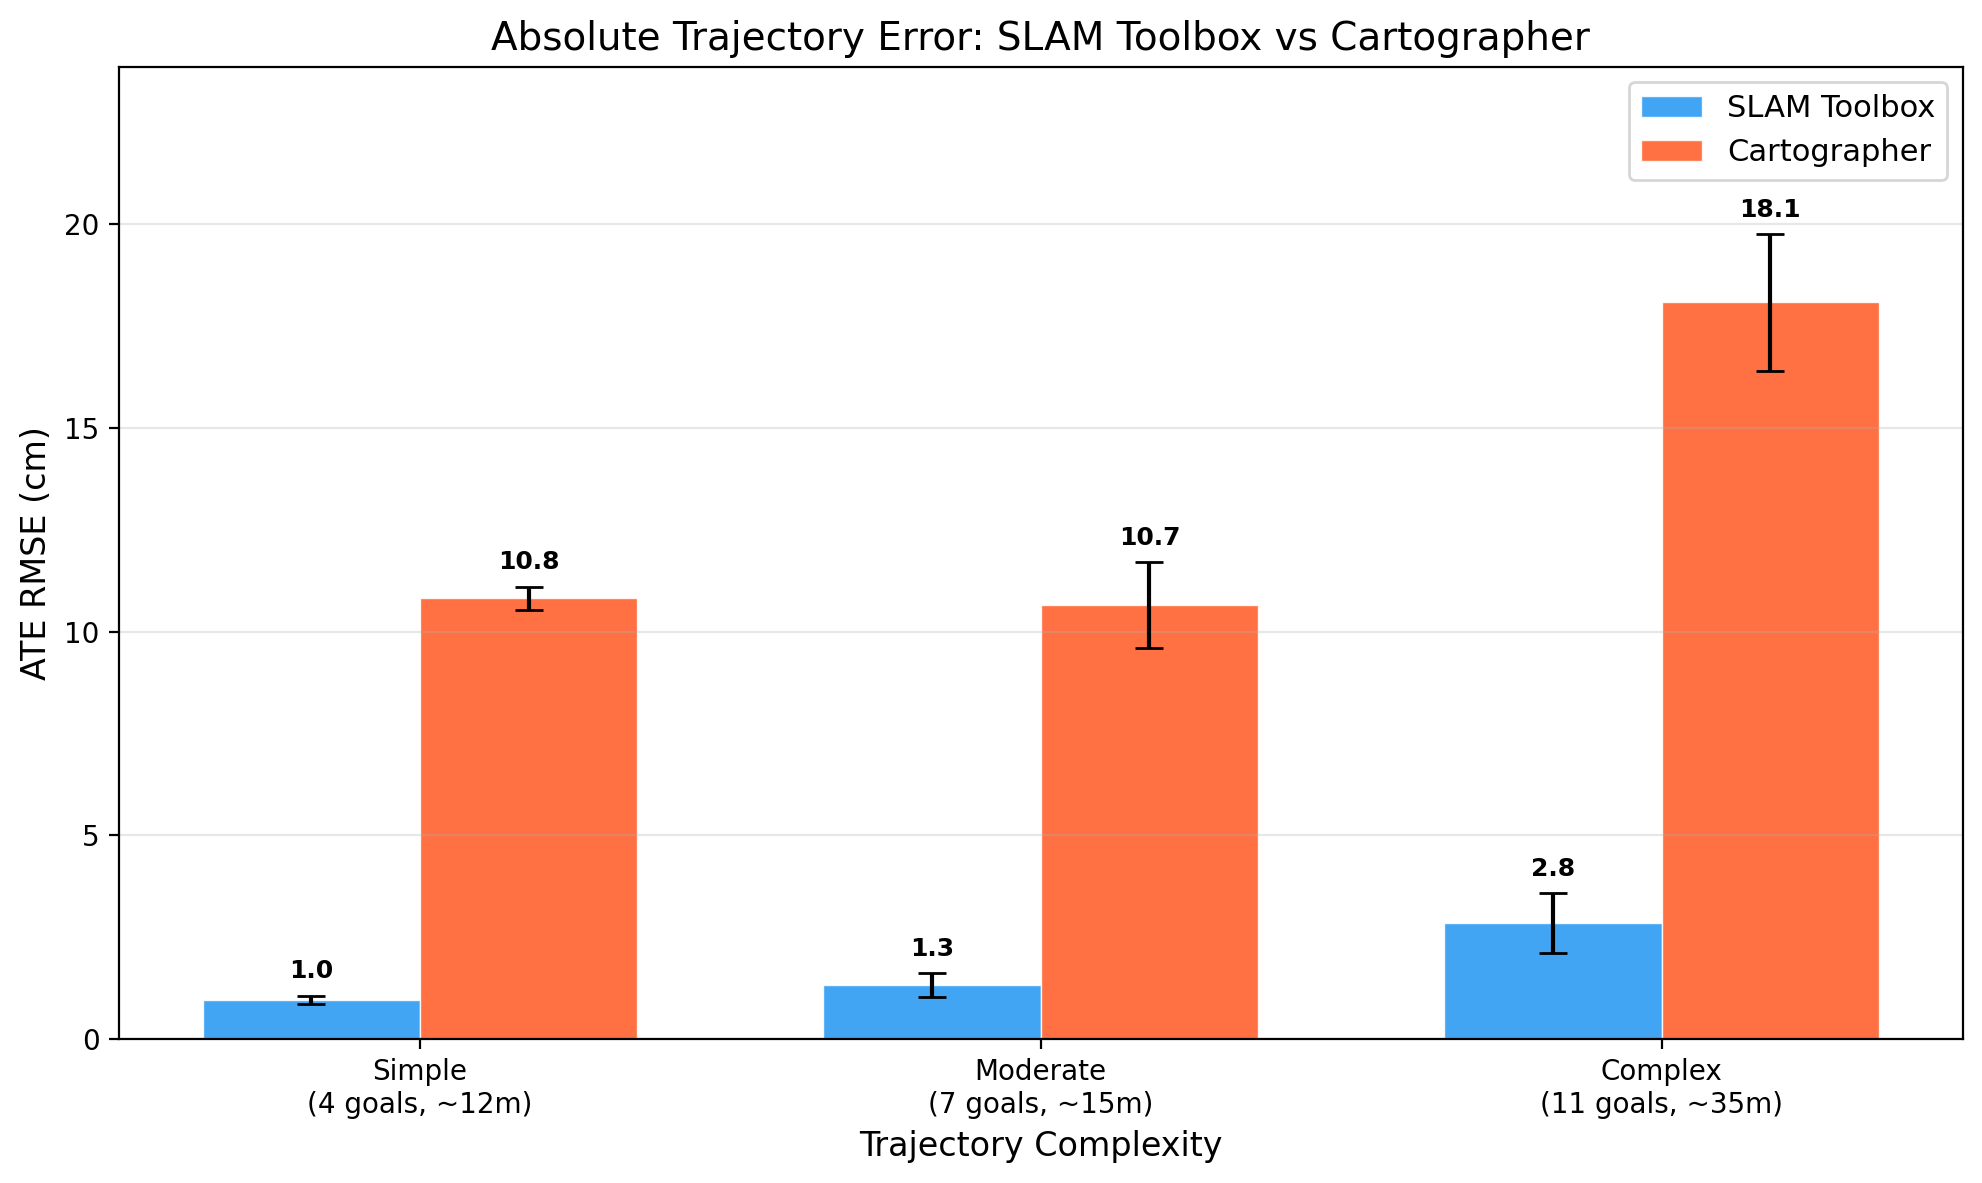
\includegraphics[width=0.85\textwidth]{ate_comparison.png}
\caption{Absolute Trajectory Error comparison across goal sets. Error bars indicate standard deviation across 3 runs. SLAM Toolbox achieves consistently lower ATE across all complexity levels.}
\label{fig:ate_comparison}
\end{figure}

SLAM Toolbox achieves ATE RMSE values of 0.96--2.84\,cm across the three goal sets, while Cartographer produces ATE RMSE values of 10.82--18.09\,cm. The accuracy ratio ranges from 11.3$\times$ on the simple trajectory to 6.4$\times$ on the complex trajectory, with the gap narrowing as complexity increases. Figure~\ref{fig:accuracy_ratio} illustrates this trend.

\begin{figure}[htbp]
\centering
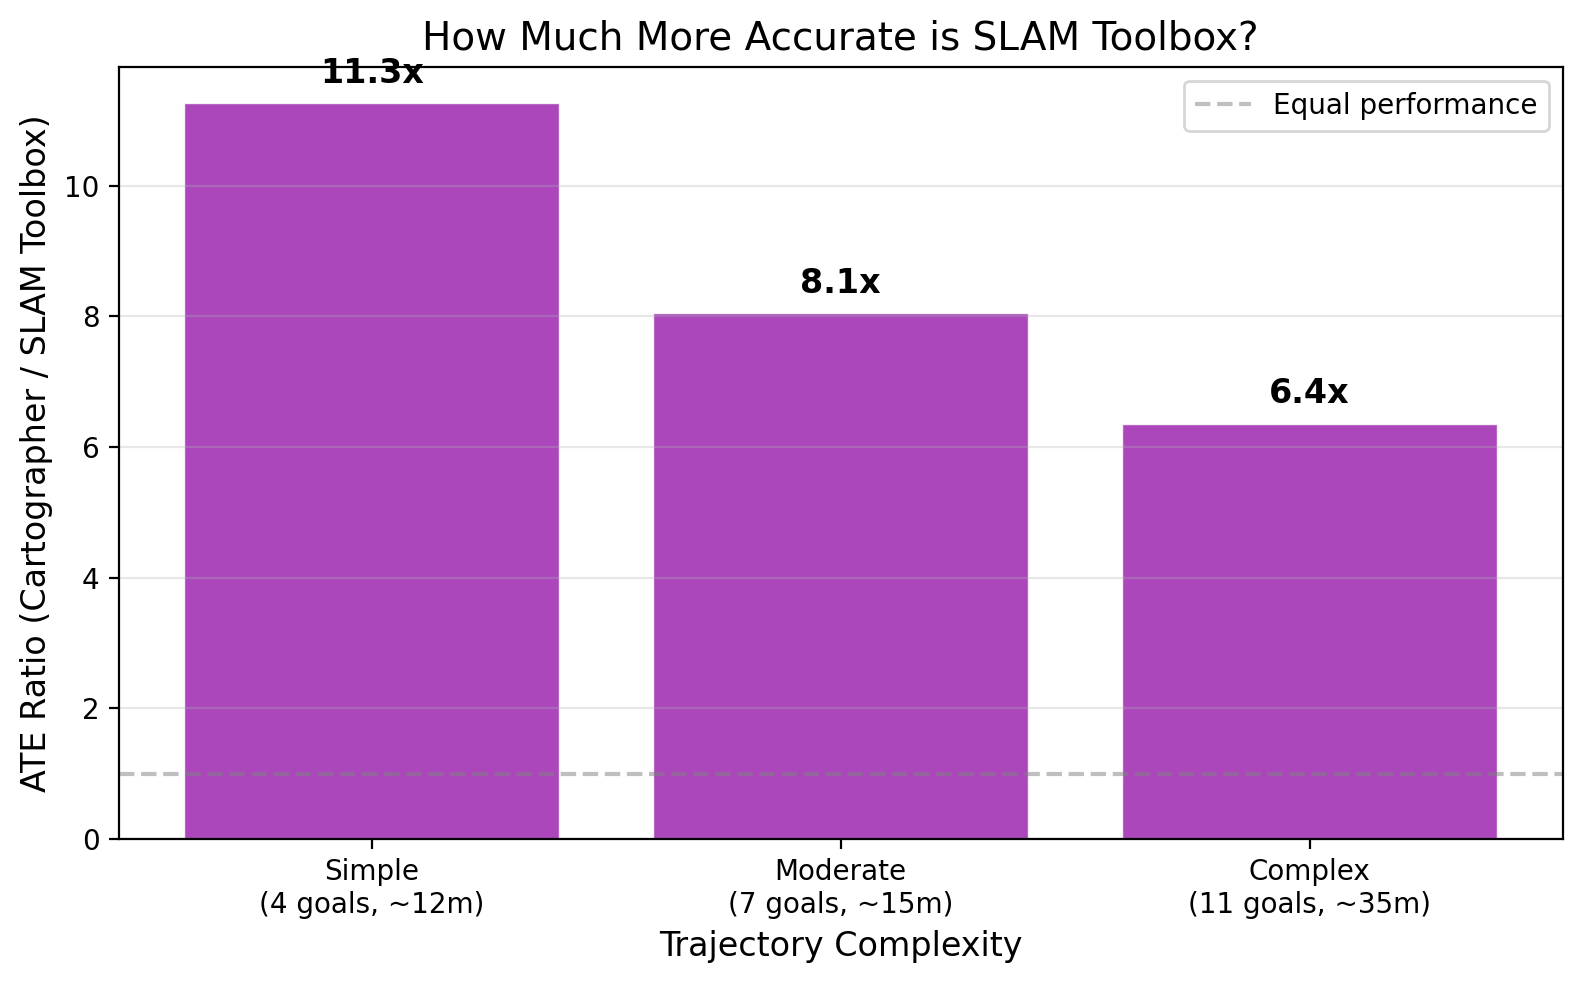
\includegraphics[width=0.7\textwidth]{accuracy_ratio.png}
\caption{ATE accuracy ratio (Cartographer / SLAM Toolbox) across goal sets. The ratio decreases from 11.3$\times$ to 6.4$\times$ as trajectory complexity increases.}
\label{fig:accuracy_ratio}
\end{figure}

Table~\ref{tab:ate_individual} presents the individual run ATE values, showing the consistency of results across repetitions.

\begin{table}[htbp]
\centering
\caption{Individual run ATE RMSE values (cm).}
\label{tab:ate_individual}
\begin{tabular}{lcccc}
\toprule
\textbf{Algorithm} & \textbf{Goal Set} & \textbf{Run 1} & \textbf{Run 2} & \textbf{Run 3} \\
\midrule
SLAM Toolbox & Simple & 1.05 & 0.85 & 0.99 \\
SLAM Toolbox & Moderate & 1.44 & 0.99 & 1.54 \\
SLAM Toolbox & Complex & 2.42 & 2.42 & 3.69 \\
\midrule
Cartographer & Simple & 11.13 & 10.76 & 10.57 \\
Cartographer & Moderate & 11.04 & 9.47 & 11.46 \\
Cartographer & Complex & 16.21 & 18.56 & 19.48 \\
\bottomrule
\end{tabular}
\end{table}

The ATE distributions are further visualized as box plots in Figure~\ref{fig:ate_boxplots}, showing the spread of individual measurements for each configuration.

\begin{figure}[htbp]
\centering
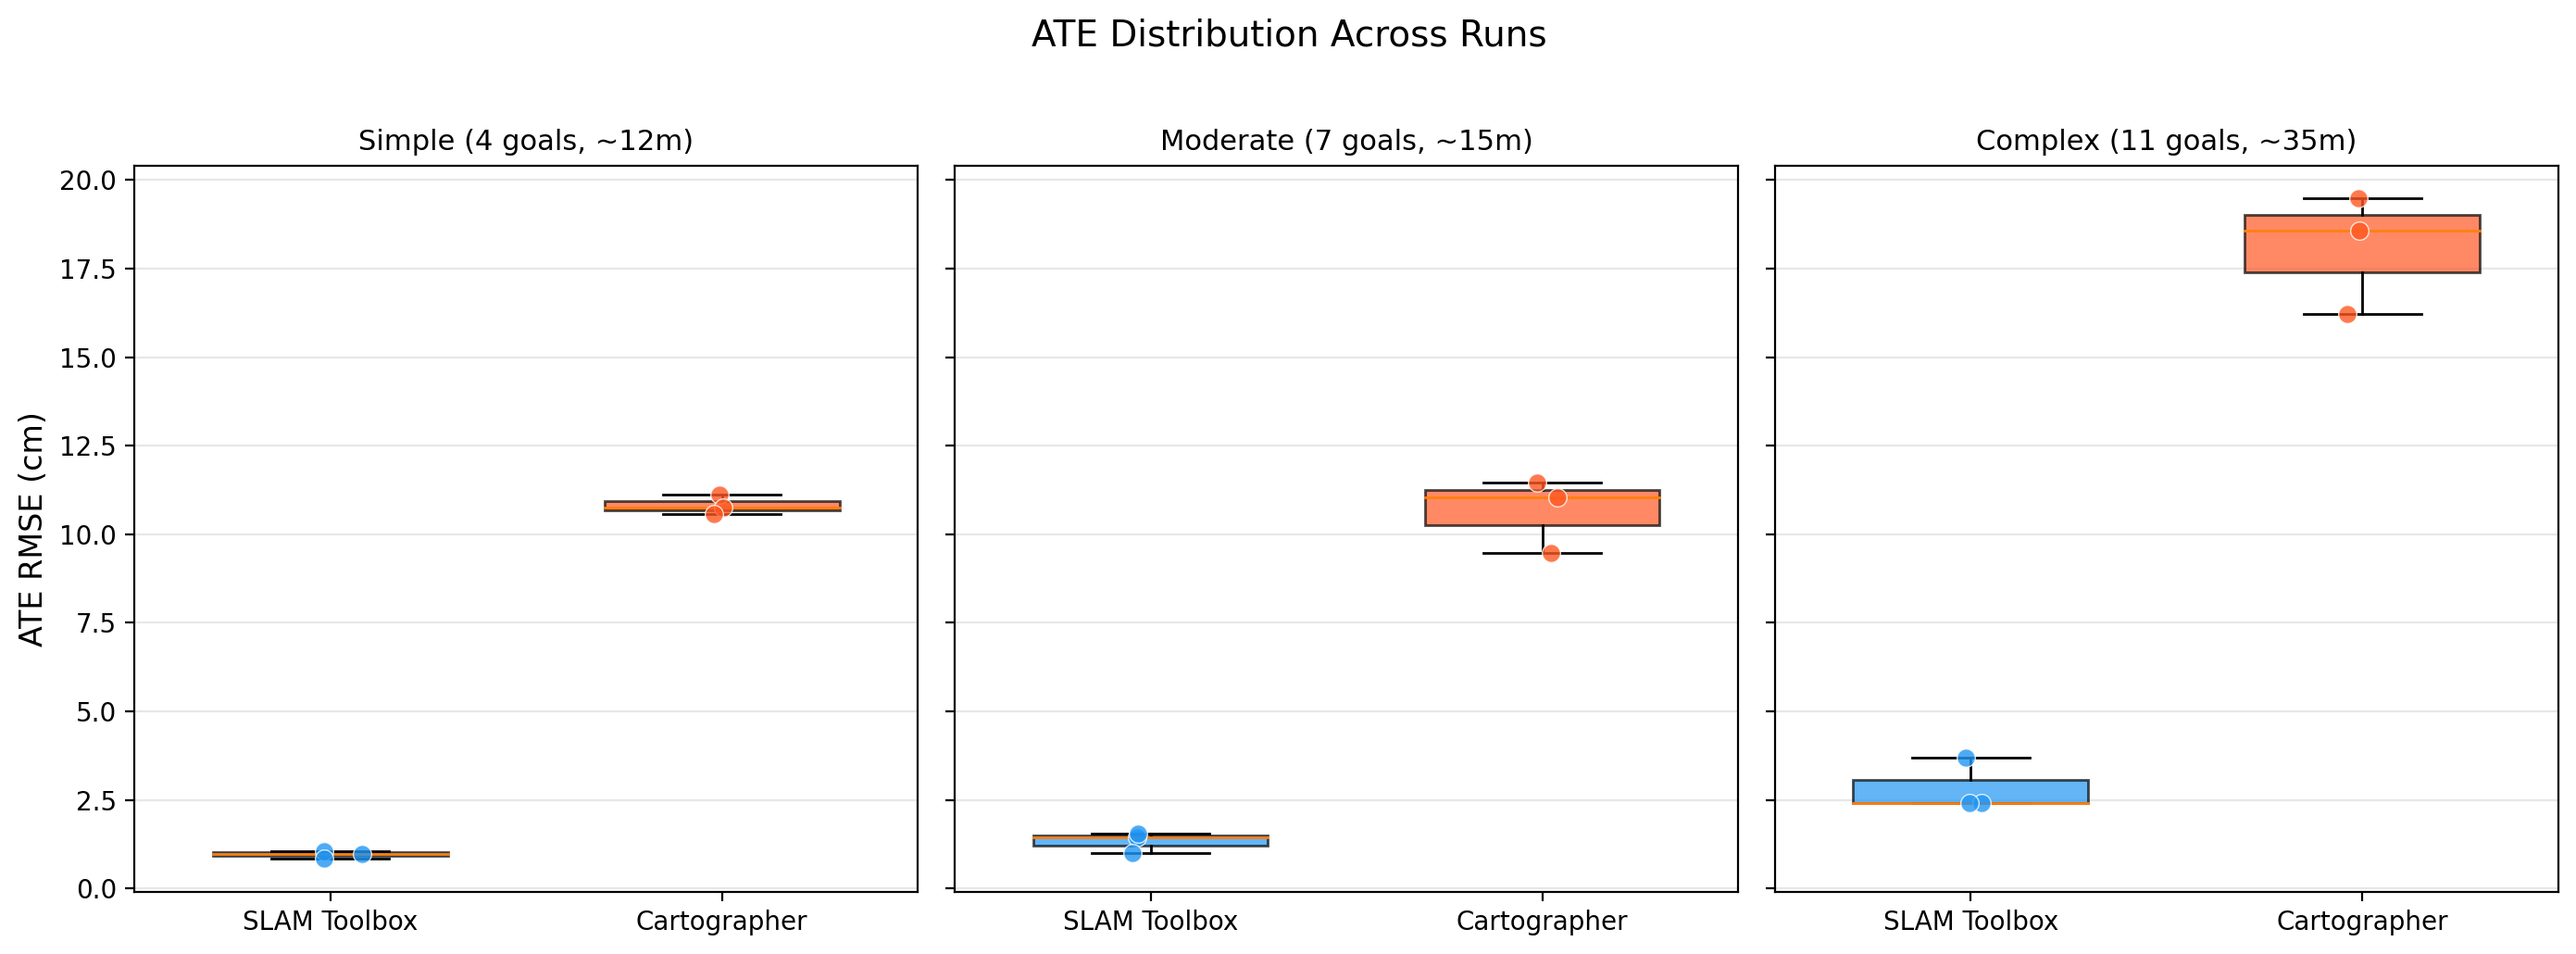
\includegraphics[width=0.95\textwidth]{ate_boxplots.png}
\caption{Box plots of ATE RMSE distributions for each algorithm across the three goal sets. Individual data points are overlaid.}
\label{fig:ate_boxplots}
\end{figure}

\section{SLAM Accuracy: Relative Pose Error}

The Relative Pose Error captures local accuracy independent of global drift. Table~\ref{tab:rpe_results} presents the RPE RMSE results, and Figure~\ref{fig:rpe_comparison} shows the visual comparison.

\begin{table}[htbp]
\centering
\caption{Relative Pose Error RMSE (cm): mean across 3 runs.}
\label{tab:rpe_results}
\begin{tabular}{lccc}
\toprule
\textbf{Algorithm} & \textbf{Simple} & \textbf{Moderate} & \textbf{Complex} \\
\midrule
SLAM Toolbox & 0.56 & 0.57 & 0.68 \\
Cartographer & 0.93 & 1.15 & 2.02 \\
\midrule
\textbf{Ratio (CG/ST)} & \textbf{1.7$\times$} & \textbf{2.0$\times$} & \textbf{3.0$\times$} \\
\bottomrule
\end{tabular}
\end{table}

\begin{figure}[htbp]
\centering
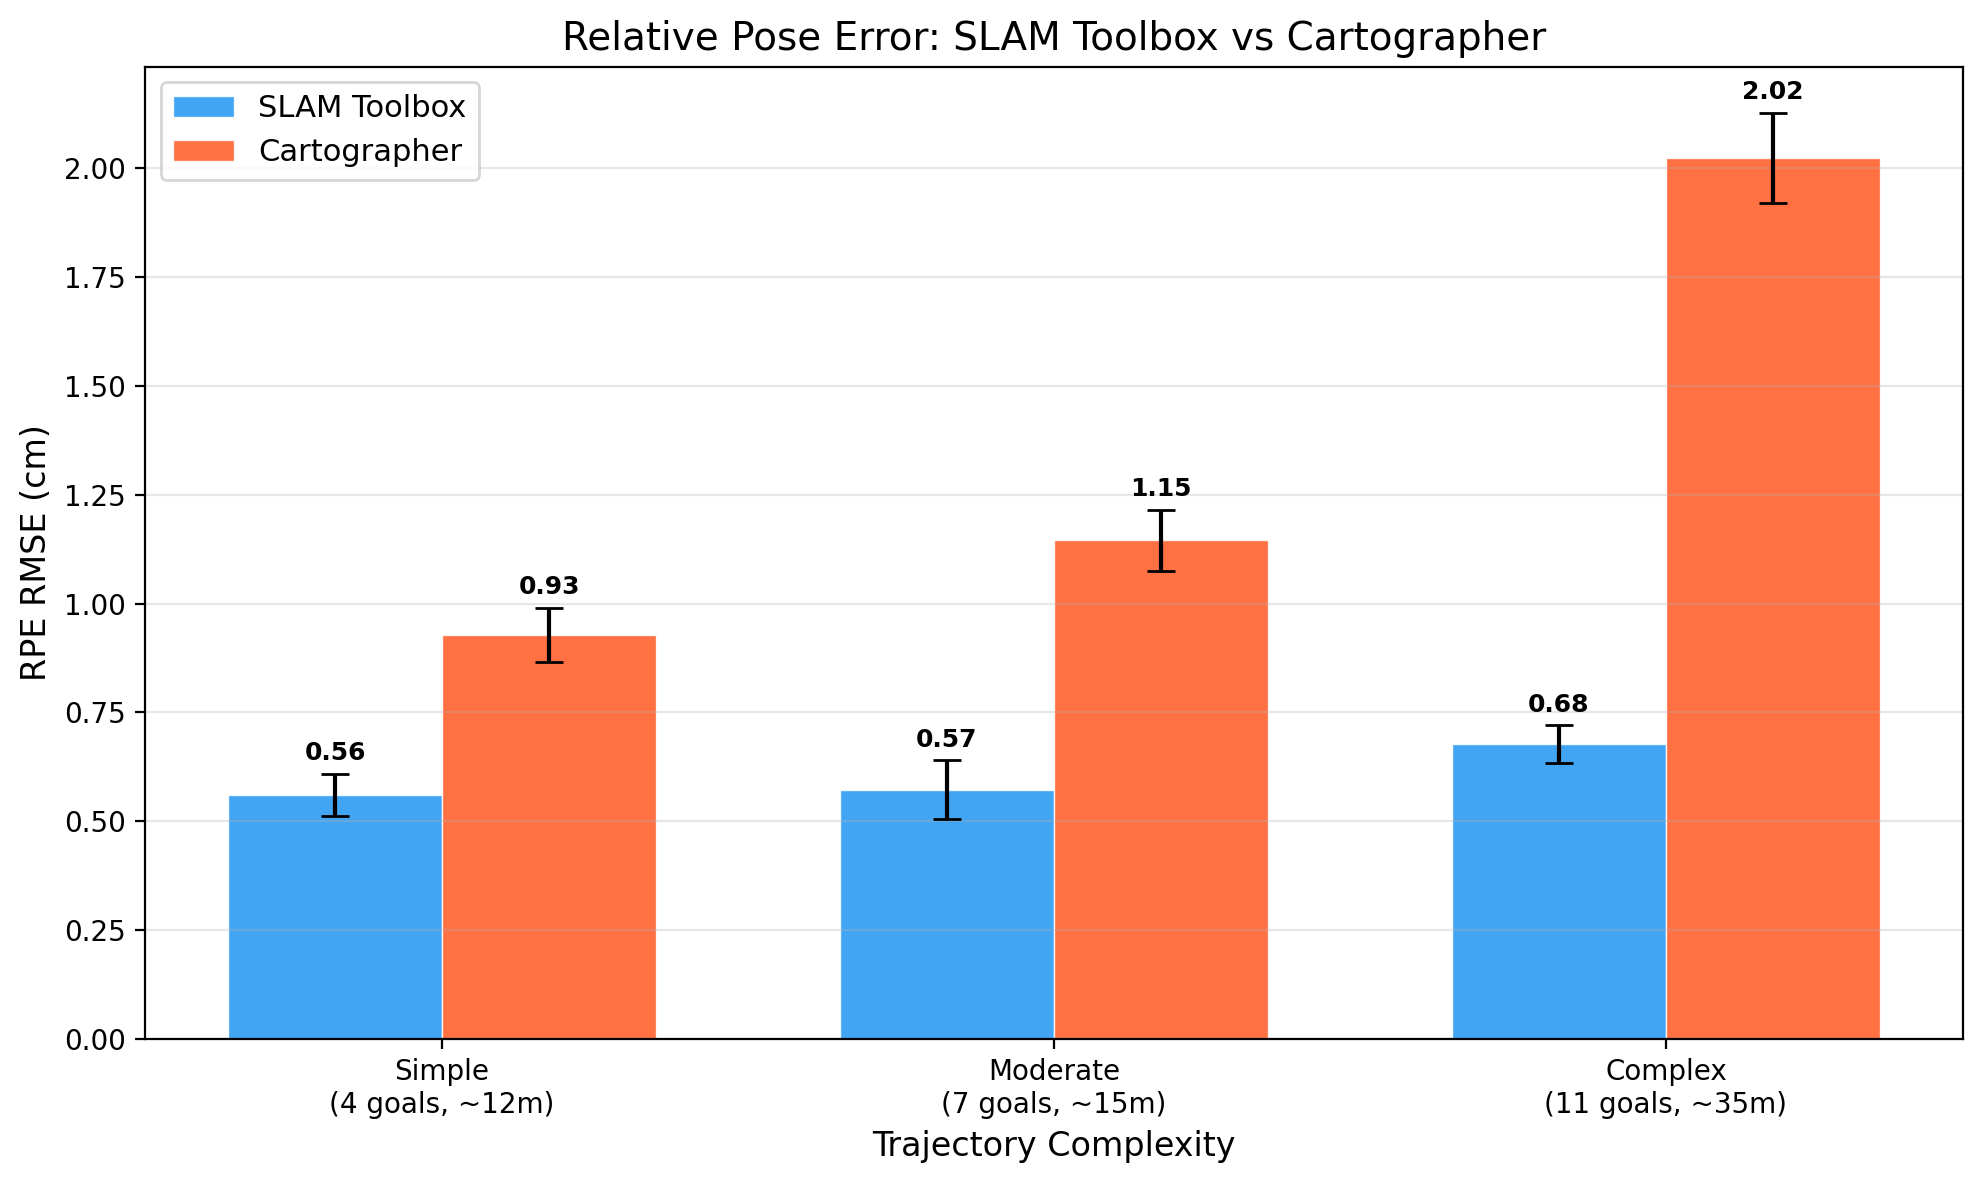
\includegraphics[width=0.85\textwidth]{rpe_comparison.png}
\caption{Relative Pose Error comparison across goal sets.}
\label{fig:rpe_comparison}
\end{figure}

The RPE ratio between algorithms (1.7--3.0$\times$) is notably smaller than the ATE ratio (6.4--11.3$\times$). This indicates that the primary accuracy difference lies in \emph{global consistency} rather than \emph{local scan matching quality}. Both algorithms produce reasonable local pose estimates, but SLAM Toolbox maintains better global trajectory coherence, likely due to differences in their pose graph optimization strategies.

\section{Navigation Time Analysis}

Table~\ref{tab:time_results} presents the mean total mission time for each configuration, and Figure~\ref{fig:time_comparison} provides a visual comparison.

\begin{table}[htbp]
\centering
\caption{Total navigation time (seconds): mean $\pm$ standard deviation across 3 runs.}
\label{tab:time_results}
\begin{tabular}{lccc}
\toprule
\textbf{Algorithm} & \textbf{Simple} & \textbf{Moderate} & \textbf{Complex} \\
\midrule
SLAM Toolbox & $45.9 \pm 2.2$ & $70.9 \pm 0.9$ & $156.4 \pm 0.2$ \\
Cartographer & $48.9 \pm 0.6$ & $74.5 \pm 3.0$ & $156.8 \pm 2.3$ \\
\bottomrule
\end{tabular}
\end{table}

\begin{figure}[htbp]
\centering
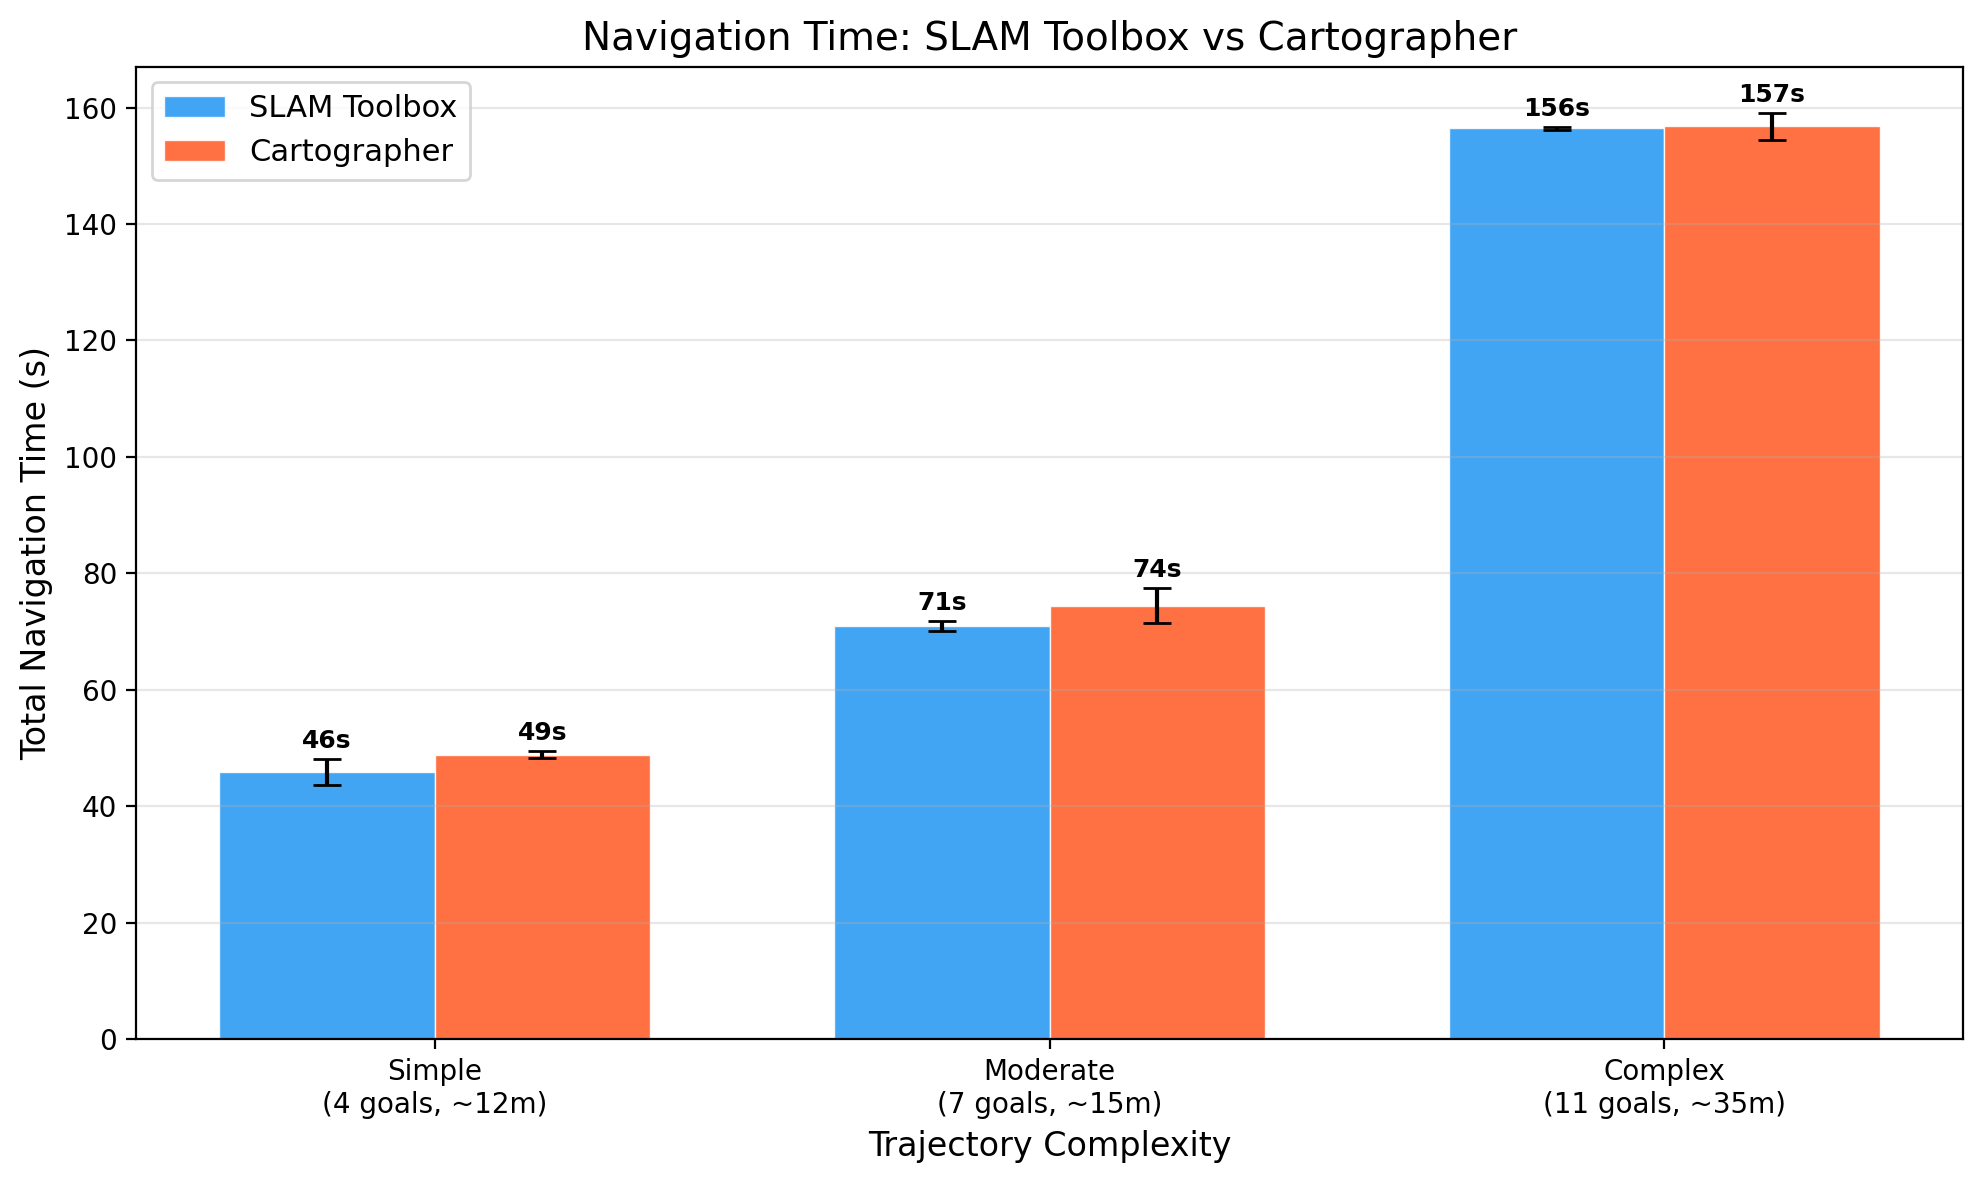
\includegraphics[width=0.85\textwidth]{time_comparison.png}
\caption{Navigation time comparison across goal sets.}
\label{fig:time_comparison}
\end{figure}

Navigation times are remarkably similar between algorithms, with differences of less than 7\% across all goal sets. On the complex trajectory, the times are nearly identical (156.4\,s vs.\ 156.8\,s). This finding reinforces the observation that the substantial SLAM accuracy difference does not translate to a measurable navigation performance difference within this experimental context.

\section{Scaling Behavior}

Figure~\ref{fig:ate_scaling} shows how ATE RMSE scales with approximate trajectory length for both algorithms.

\begin{figure}[htbp]
\centering
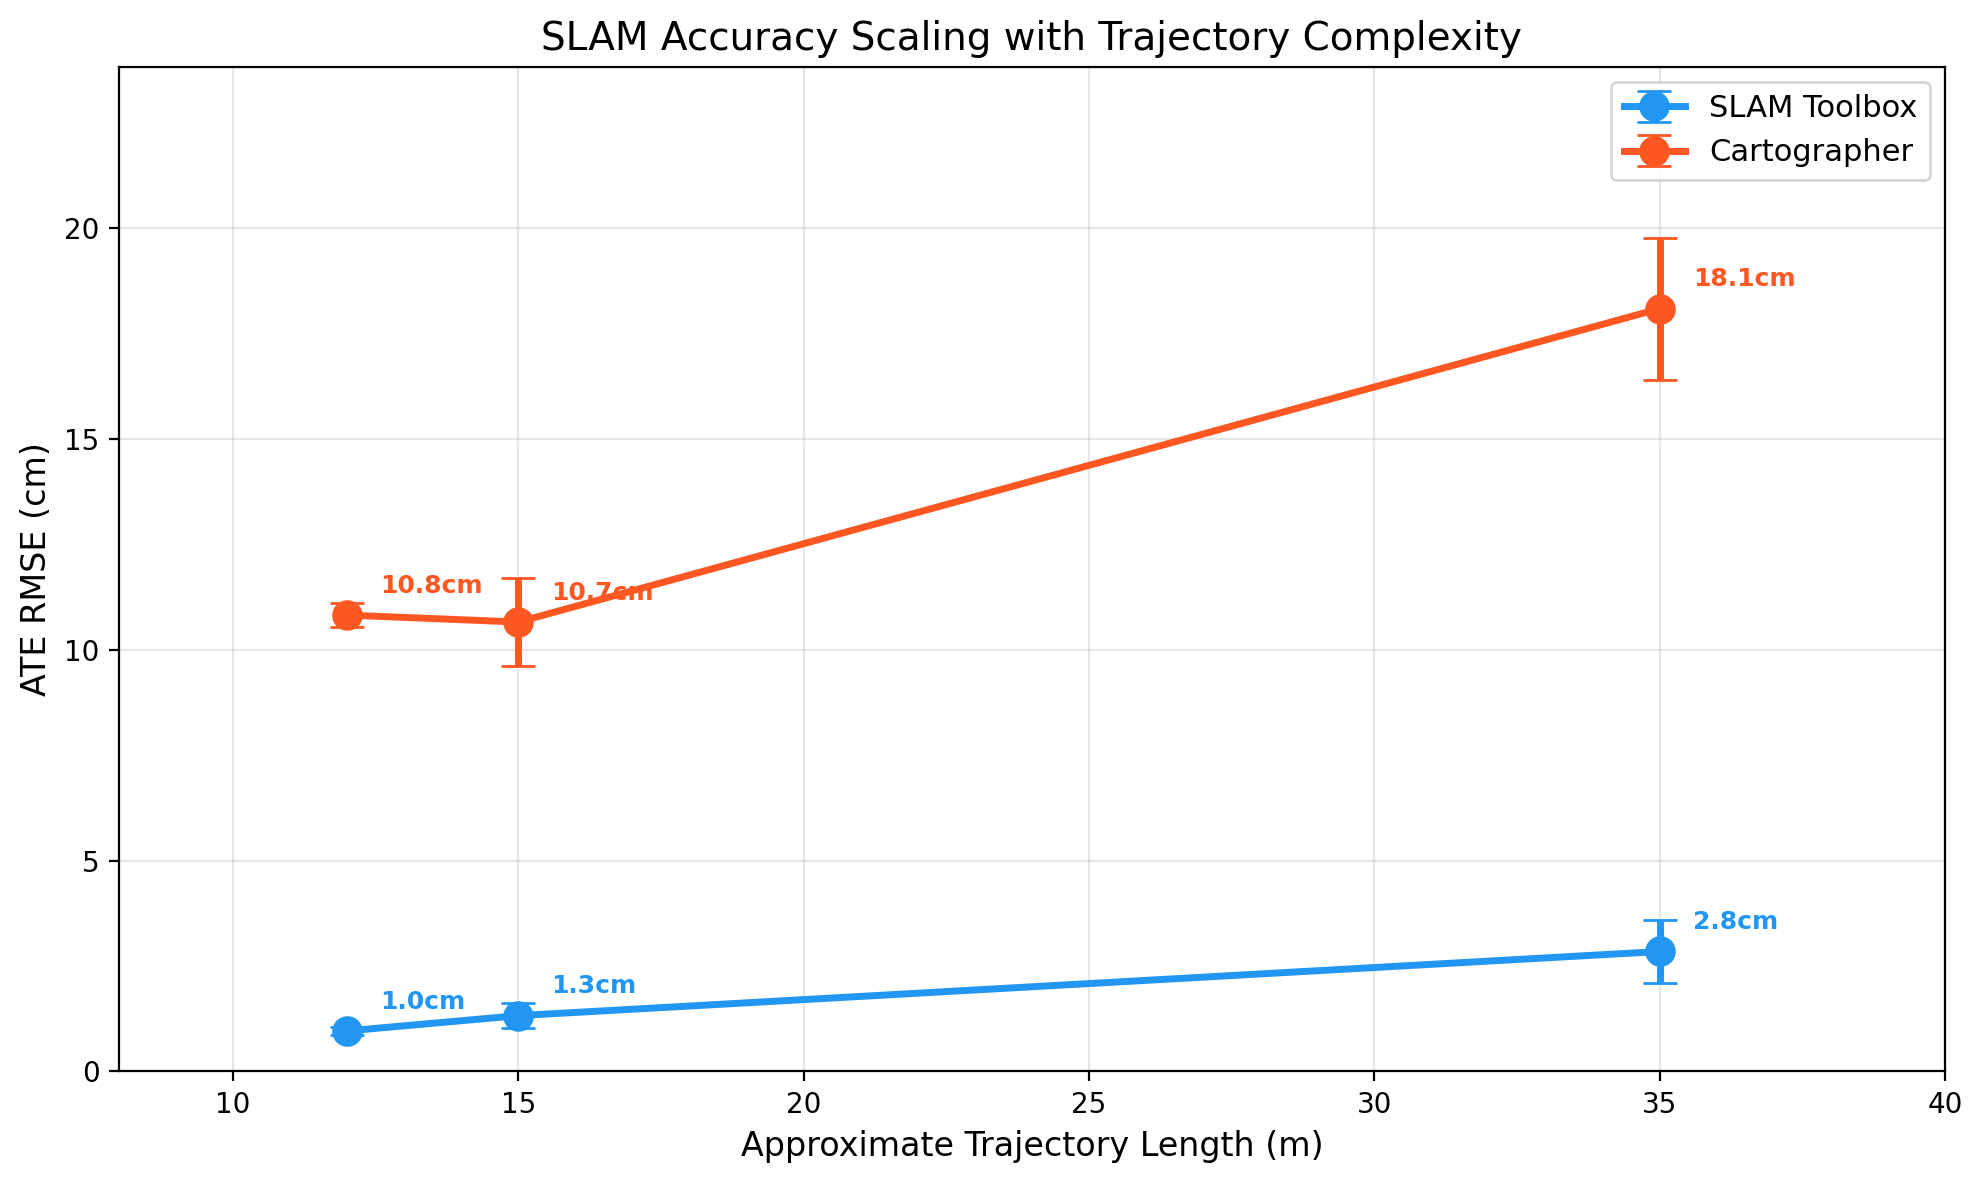
\includegraphics[width=0.85\textwidth]{ate_scaling.png}
\caption{ATE RMSE as a function of trajectory length. Both algorithms show approximately linear error growth, but from substantially different baselines. Error bars indicate standard deviation.}
\label{fig:ate_scaling}
\end{figure}

Both algorithms exhibit approximately linear ATE growth with trajectory length, consistent with the expected drift accumulation in SLAM systems. SLAM Toolbox's error grows from 0.96\,cm at 12\,m to 2.84\,cm at 35\,m---a rate of approximately 0.08\,cm per meter of travel. Cartographer's error grows from 10.82\,cm to 18.09\,cm over the same range---a rate of approximately 0.32\,cm per meter, roughly 4$\times$ the drift rate of SLAM Toolbox.

Notably, Cartographer's ATE on the moderate trajectory (10.65\,cm) is slightly \emph{lower} than on the simple trajectory (10.82\,cm), suggesting some run-to-run variability in its baseline accuracy rather than a strictly monotonic degradation.

\section{Run-to-Run Consistency}

Figure~\ref{fig:individual_runs_scatter} displays all 18 individual ATE measurements, providing a view of both between-algorithm and within-algorithm variability.

\begin{figure}[htbp]
\centering
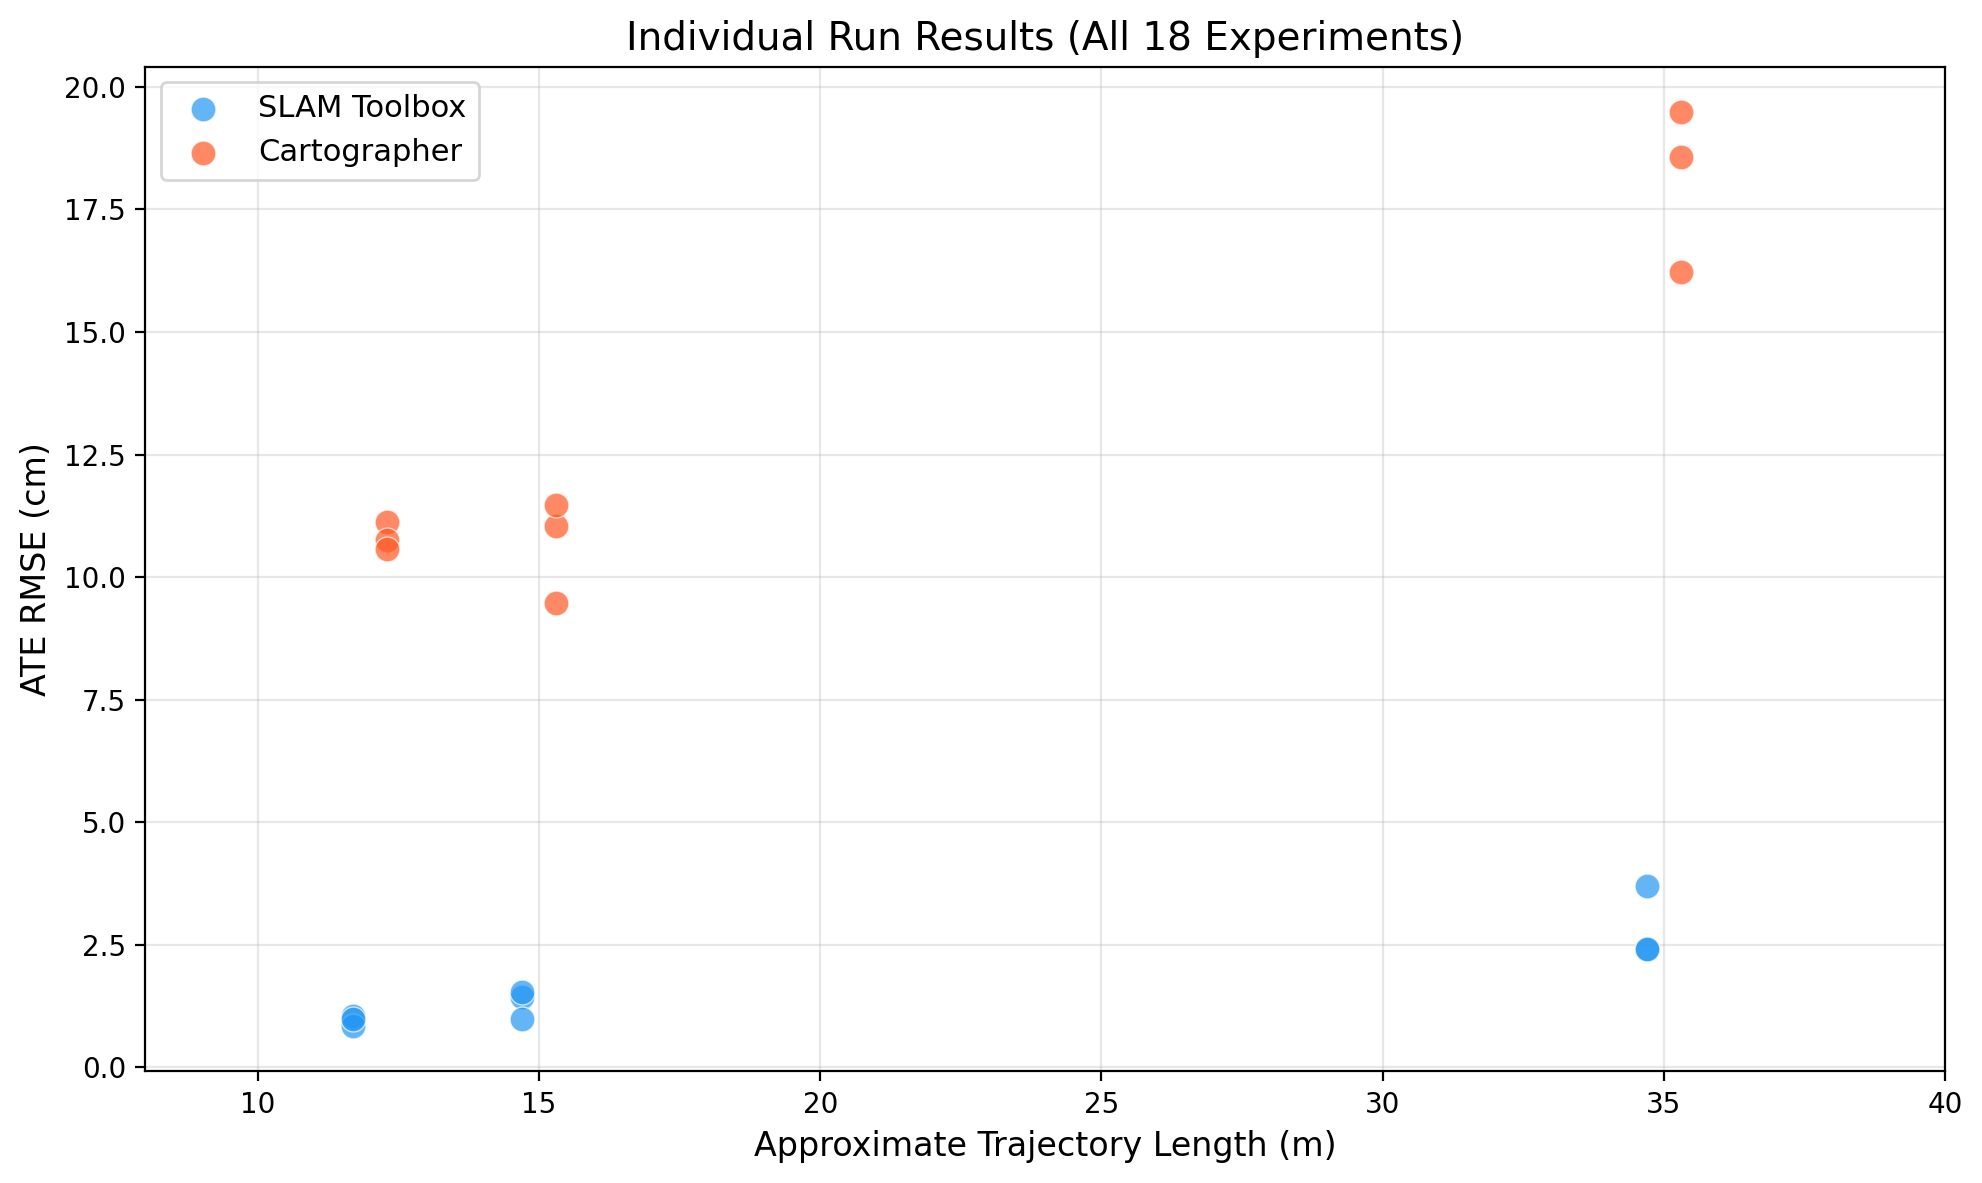
\includegraphics[width=0.85\textwidth]{individual_runs_scatter.png}
\caption{Individual run ATE RMSE values for all 18 experiments. Points are jittered horizontally for visibility.}
\label{fig:individual_runs_scatter}
\end{figure}

SLAM Toolbox demonstrates high consistency on the simple and moderate trajectories (standard deviations of 0.10\,cm and 0.29\,cm, respectively), with somewhat more variability on the complex trajectory (0.74\,cm). Cartographer shows similar consistency on the simple trajectory (0.29\,cm) but increasing variability with complexity (1.05\,cm and 1.68\,cm for moderate and complex trajectories). This pattern suggests that longer, more complex trajectories introduce more stochastic variation in SLAM performance, particularly for Cartographer.

\section{Summary of Results}

Table~\ref{tab:consolidated_results} provides a consolidated view of all key metrics.

\begin{table}[htbp]
\centering
\caption{Consolidated experimental results (mean $\pm$ std, $n=3$).}
\label{tab:consolidated_results}
\begin{tabular}{llccccc}
\toprule
\textbf{Algorithm} & \textbf{Goals} & \textbf{Success} & \textbf{ATE (cm)} & \textbf{RPE (cm)} & \textbf{Time (s)} \\
\midrule
SLAM Toolbox & Simple & 100\% & $0.96 \pm 0.10$ & 0.56 & $45.9$ \\
SLAM Toolbox & Moderate & 100\% & $1.32 \pm 0.29$ & 0.57 & $70.9$ \\
SLAM Toolbox & Complex & 100\% & $2.84 \pm 0.74$ & 0.68 & $156.4$ \\
Cartographer & Simple & 100\% & $10.82 \pm 0.29$ & 0.93 & $48.9$ \\
Cartographer & Moderate & 100\% & $10.65 \pm 1.05$ & 1.15 & $74.5$ \\
Cartographer & Complex & 100\% & $18.09 \pm 1.68$ & 2.02 & $156.8$ \\
\bottomrule
\end{tabular}
\end{table}

\chapter{Discussion}
\label{ch:discussion}

This chapter interprets the experimental results in the context of our research questions, analyzes the observed accuracy--utility gap, explores algorithmic explanations for the performance differences, discusses practical implications, and acknowledges limitations.

\section{Answering the Research Questions}

\subsection{RQ1: SLAM Accuracy Comparison}

\emph{How do SLAM Toolbox and Cartographer compare in SLAM accuracy across trajectories of varying complexity?}

The results provide a clear answer: SLAM Toolbox achieves substantially higher trajectory accuracy than Cartographer across all three complexity levels. The ATE RMSE ratio ranges from 11.3$\times$ on the simple trajectory to 6.4$\times$ on the complex trajectory, consistently favoring SLAM Toolbox. In absolute terms, SLAM Toolbox maintains sub-centimeter accuracy on short trajectories (0.96\,cm on the simple goal set) and below 3\,cm even on the longest trajectory (2.84\,cm on the complex goal set with approximately 35\,m of travel).

The RPE analysis reveals that the accuracy gap is primarily in global trajectory consistency (ATE) rather than local pose estimation (RPE). RPE ratios of 1.7--3.0$\times$ are notably smaller than the ATE ratios, indicating that both algorithms achieve reasonable local scan matching accuracy but differ in how effectively they maintain global coherence through loop closure and pose graph optimization.

Both algorithms exhibit approximately linear error growth with trajectory length, which is consistent with the expected behavior of SLAM systems where drift accumulates between loop closure opportunities. SLAM Toolbox's drift rate (approximately 0.08\,cm/m) is roughly four times lower than Cartographer's (approximately 0.32\,cm/m), suggesting more effective continuous drift correction.

\subsection{RQ2: Accuracy and Navigation Success}

\emph{Does SLAM accuracy predict navigation success rate and efficiency?}

The most striking finding of this study is the complete decoupling of SLAM accuracy from navigation success within our experimental conditions. Despite a 6--11$\times$ difference in ATE, both algorithms achieve identical 100\% navigation success rates across all goal sets and all repetitions. Navigation mission times are also nearly identical, differing by less than 7\% between algorithms.

This result has a straightforward explanation: the Nav2 goal checker uses an XY tolerance of 0.25\,m (25\,cm) to determine whether a goal has been reached. Cartographer's worst-case ATE of approximately 18\,cm remains well within this tolerance. More importantly, the DWB local controller continuously replans based on the current pose estimate, effectively compensating for global drift as long as the robot remains within the costmap and the local scan matching provides sufficient accuracy for path following.

This finding does not imply that SLAM accuracy is irrelevant---rather, it demonstrates that for navigation tasks in bounded indoor environments with the default Nav2 tolerances, even the less accurate algorithm provides sufficient localization. The accuracy difference would likely become task-relevant in scenarios requiring tighter positioning tolerances, such as precision docking, manipulation, or multi-robot coordination.

\subsection{RQ3: Scaling with Complexity}

\emph{How do the algorithms scale as trajectory length and complexity increase?}

Both algorithms show degradation with increasing trajectory complexity, but with different characteristics. SLAM Toolbox's ATE grows from 0.96\,cm to 2.84\,cm (a 3.0$\times$ increase) as the path length increases from approximately 12\,m to 35\,m (a 2.9$\times$ increase), showing nearly linear scaling. Cartographer's ATE grows from 10.82\,cm to 18.09\,cm (a 1.7$\times$ increase), showing sub-linear scaling relative to path length.

Interestingly, the accuracy \emph{ratio} between algorithms decreases with complexity (11.3$\times$ $\rightarrow$ 8.1$\times$ $\rightarrow$ 6.4$\times$). This convergence could be attributed to Cartographer's loop closure mechanism becoming more effective on longer trajectories where the robot revisits more areas, or to SLAM Toolbox's error growth rate eventually catching up at larger scales.

Run-to-run variability also increases with trajectory complexity for both algorithms, with Cartographer showing higher variance. This is consistent with the stochastic nature of loop closure detection and the increased number of decisions the algorithms must make on longer trajectories.

\section{The Accuracy--Utility Gap}

The central finding of this thesis---that a substantial SLAM accuracy difference produces no measurable navigation performance difference---warrants deeper analysis. We term this the \emph{accuracy--utility gap}: the disparity between what accuracy benchmarks measure and what task performance requires.

Traditional SLAM benchmarks such as TUM RGB-D \citep{sturm2012benchmark} and KITTI \citep{geiger2013kitti} evaluate trajectory accuracy because it is a well-defined, sensor-agnostic metric that captures the fundamental quality of the SLAM solution. However, accuracy is a \emph{proxy metric} for the actual goal of enabling robot autonomy. Our results demonstrate that this proxy can be misleading when comparing algorithms for deployment: an algorithm with 11$\times$ worse accuracy may perform identically on the actual task.

This finding has several implications for the SLAM evaluation community:

\begin{enumerate}
\item \textbf{Accuracy thresholds matter more than accuracy values.} Rather than comparing ATE values directly, practitioners should identify the accuracy threshold required by their application and verify that candidate algorithms meet it. For Nav2-based navigation with default tolerances, an ATE below approximately 25\,cm appears sufficient.

\item \textbf{Task-driven evaluation provides complementary information.} ATE and RPE remain valuable for understanding algorithm capabilities, but should be supplemented with task-level metrics when the goal is algorithm selection for deployment.

\item \textbf{System-level factors may dominate.} The navigation stack's ability to compensate for SLAM errors through replanning, local control, and goal tolerance means that system-level design choices (tolerance settings, controller tuning, recovery behaviors) may have more impact on task success than the choice of SLAM algorithm.
\end{enumerate}

\section{Algorithmic Analysis}

Several factors may explain SLAM Toolbox's consistent accuracy advantage:

\textbf{Continuous pose graph optimization.} SLAM Toolbox maintains and optimizes a single pose graph throughout the mapping session, with each scan insertion potentially triggering local optimization. Cartographer, by contrast, groups scans into submaps and optimizes at a coarser granularity (every 90 nodes in our configuration). This difference in optimization frequency may allow SLAM Toolbox to correct drift more promptly.

\textbf{Default parameter suitability.} The published default parameters for each algorithm were designed for different reference platforms. SLAM Toolbox was developed within the ROS~2 ecosystem specifically for mobile robot applications, while Cartographer originated at Google for large-scale indoor mapping with different sensor configurations. The default parameters may favor the smaller, slower rover platform used in our experiments.

\textbf{Scan matching strategy.} SLAM Toolbox uses correlative scan matching followed by Ceres refinement against a continuously updated map, while Cartographer matches scans against local submaps with a separate correlative pre-matching step. The continuous map approach may provide richer context for scan matching, reducing per-scan drift.

We emphasize that these are hypotheses based on the algorithmic descriptions and observed behavior. A definitive explanation would require controlled ablation studies isolating individual algorithm components, which is beyond the scope of this thesis.

\section{Practical Implications}

Based on our findings, we offer the following guidance for practitioners selecting between SLAM Toolbox and Cartographer for 2D LiDAR applications:

\begin{itemize}
\item For \textbf{standard navigation tasks} in indoor environments where goal tolerances are on the order of tens of centimeters, either algorithm is suitable. The choice may then be driven by non-accuracy factors such as computational resource availability, API familiarity, and community support.

\item For \textbf{accuracy-critical applications} such as precision docking, fleet management requiring consistent global coordinates, or mapping for subsequent localization, SLAM Toolbox's superior ATE makes it the preferred choice under default configurations.

\item For applications where \textbf{parameter tuning is feasible}, the accuracy gap may narrow significantly. Prior work on this project demonstrated that Optuna-based hyperparameter optimization reduced Cartographer's ATE from approximately 10\,cm to below 1\,cm on short trajectories, suggesting that Cartographer's potential is constrained by its default parameters rather than fundamental algorithmic limitations.
\end{itemize}

\section{Limitations}

This study has several limitations that should be considered when interpreting the results:

\begin{enumerate}
\item \textbf{Simulation-only evaluation.} All experiments were conducted in the Gazebo simulator, which provides idealized sensor data without the noise, calibration errors, and environmental variability encountered in real-world deployments. The absence of sensor noise likely benefits both algorithms but may disproportionately affect the relative comparison.

\item \textbf{Single environment.} Experiments used a single 10$\times$10\,m room environment. Different environment types (long corridors, open areas, symmetric rooms) may expose different algorithm behaviors, particularly regarding loop closure performance and scan matching degeneracy.

\item \textbf{Default parameters.} Both algorithms were evaluated with published default parameters. Algorithm-specific tuning could significantly alter the relative performance, as demonstrated by preliminary Optuna experiments on this project.

\item \textbf{Single navigation configuration.} Only one Nav2 configuration (NavfnPlanner + DWB controller) was tested. Different planners or controllers may interact differently with SLAM accuracy variations.

\item \textbf{Limited repetitions.} Three repetitions per configuration provide a measure of variability but limit statistical power for formal hypothesis testing. A larger sample size would strengthen the conclusions.

\item \textbf{No sensor degradation.} The simulator provides perfect odometry and noise-free laser scans. Real deployments contend with wheel slip, encoder noise, and LiDAR artifacts that may differentially affect the two algorithms.

\item \textbf{2D LiDAR only.} The comparison is limited to 2D LiDAR SLAM. Both algorithms support additional sensor modalities (3D LiDAR, IMU) that were not evaluated.
\end{enumerate}

\section{Threats to Validity}

\textbf{Internal validity.} The use of simulation ensures consistent experimental conditions across runs. However, the simulation's physics engine introduces its own approximations that may not perfectly represent real robot behavior. The automated process cleanup between runs mitigates the risk of state leakage between experiments.

\textbf{External validity.} Results obtained in simulation with a specific robot model, sensor configuration, and environment may not generalize to other platforms, environments, or real-world conditions. The single-environment design limits the breadth of conclusions about algorithm behavior across diverse scenarios.

\textbf{Construct validity.} ATE RMSE is an established metric for SLAM trajectory accuracy, but it is a single-number summary that may not capture all aspects of SLAM quality (e.g., map accuracy, consistency of loop closures, computational efficiency). Navigation success rate is a coarse binary metric that may not capture subtle differences in navigation quality such as path smoothness or recovery frequency.

\chapter{Conclusion and Future Work}
\label{ch:conclusion}

\section{Summary of Contributions}

This thesis presented a navigation-driven evaluation of two prominent 2D LiDAR SLAM algorithms---SLAM Toolbox and Google Cartographer---assessed through closed-loop autonomous navigation using the Nav2 framework. The work makes the following contributions:

\begin{enumerate}
\item \textbf{A reproducible SLAM-in-the-loop evaluation framework.} We developed an open-source experimental platform integrating Gazebo Harmonic, ROS~2 Jazzy, and Nav2 that evaluates SLAM algorithms through autonomous navigation task performance. The framework includes automated experiment orchestration with batch execution, ground truth collection through a dedicated transform tree, standardized metric computation via the \texttt{evo} library, and result aggregation with visualization generation.

\item \textbf{A quantitative comparison with statistical validation.} Through 18 controlled experiments across three complexity levels with three repetitions each, we provided a statistically characterized comparison of SLAM Toolbox and Cartographer on both trajectory accuracy (ATE, RPE) and navigation performance (success rate, mission time).

\item \textbf{Empirical evidence of the accuracy--utility gap.} We demonstrated that a 6--11$\times$ difference in SLAM trajectory accuracy produces no measurable difference in navigation success or mission time within a bounded indoor environment. This finding challenges the assumption that higher SLAM accuracy directly translates to better autonomous system performance and suggests that task-driven evaluation provides important complementary information to trajectory accuracy metrics.

\item \textbf{Open-source software.} The complete experimental framework---including robot model, simulation environment, SLAM configurations, Nav2 integration, experiment orchestration, and analysis tools---is publicly available to support reproduction and extension of this work.
\end{enumerate}

\section{Key Findings}

The experimental investigation yielded four principal findings:

\textbf{Finding 1: SLAM Toolbox achieves consistently superior trajectory accuracy.} Across all three goal sets and nine repetitions per algorithm, SLAM Toolbox produced ATE RMSE values of 0.96--2.84\,cm compared to Cartographer's 10.82--18.09\,cm. The accuracy advantage is primarily in global consistency (ATE) rather than local accuracy (RPE), with RPE ratios of 1.7--3.0$\times$ compared to ATE ratios of 6.4--11.3$\times$.

\textbf{Finding 2: Navigation success is independent of SLAM accuracy in this context.} Both algorithms achieved 100\% navigation success across all 18 experiments, with nearly identical mission completion times. The Nav2 navigation stack effectively compensates for SLAM localization errors through continuous replanning and the 25\,cm goal tolerance.

\textbf{Finding 3: Both algorithms scale approximately linearly with trajectory length.} Error accumulation follows a roughly linear pattern for both algorithms, with SLAM Toolbox exhibiting a drift rate of approximately 0.08\,cm/m compared to Cartographer's 0.32\,cm/m. The accuracy gap narrows with increasing complexity, from 11.3$\times$ to 6.4$\times$.

\textbf{Finding 4: SLAM accuracy benchmarks provide incomplete deployment guidance.} The complete decoupling of trajectory accuracy from task performance in our experiments suggests that ATE comparisons alone may be insufficient for algorithm selection. Practitioners should evaluate candidate algorithms against their specific task requirements, including tolerance thresholds, environmental conditions, and computational constraints.

\section{Future Work}

Several directions for future research emerge from this work:

\textbf{Real hardware validation.} The most important extension is validating these simulation findings on physical robot hardware. Real-world experiments would introduce sensor noise, wheel slip, calibration errors, and environmental variability that may differentially affect the two algorithms. Even a limited set of real-world runs would substantially strengthen the conclusions.

\textbf{Degraded operating conditions.} Introducing controlled degradation---such as odometry noise injection, reduced LiDAR range, or sensor dropout---would test algorithm robustness and may reveal conditions under which the accuracy gap becomes navigation-relevant. The existing codebase includes infrastructure for odometry noise injection that could be activated for this purpose.

\textbf{Diverse environments.} Testing in environments that stress different SLAM capabilities---long featureless corridors (testing scan matching degeneracy), symmetric rooms (testing perceptual aliasing), and cluttered spaces (testing feature richness)---would provide a more comprehensive comparison.

\textbf{Parameter tuning study.} A systematic investigation of parameter sensitivity using automated tuning (e.g., Optuna-based optimization) would clarify whether the observed accuracy gap is fundamental to the algorithmic approaches or an artifact of default parameter settings.

\textbf{Alternative navigation configurations.} Evaluating with different Nav2 components---such as the MPPI controller, Regulated Pure Pursuit controller, or SmacPlanner---and varying goal tolerances would test the generality of the accuracy--utility gap finding.

\textbf{Longer trajectories and extended operation.} Testing with substantially longer trajectories (hundreds of meters) and extended operation times would reveal whether the observed linear drift scaling continues or whether either algorithm exhibits non-linear degradation at larger scales.

\textbf{Computational profiling.} A systematic comparison of CPU and memory utilization during SLAM and navigation would add an important practical dimension to the algorithm comparison, as computational efficiency directly affects deployability on resource-constrained robot platforms.

\textbf{Map quality evaluation.} Extending the evaluation to include map quality metrics---such as occupancy grid accuracy, structural consistency, and usability for subsequent localization---would provide a more complete picture of SLAM output quality beyond trajectory accuracy.


% ============================================================
% BIBLIOGRAPHY
% ============================================================
\bibliographystyle{plainnat}
\bibliography{references}

\end{document}
